\documentclass[
	%parspace, % Térköz bekezdések közé / Add vertical space between paragraphs
	%noindent, % Bekezdésének első sora ne legyen behúzva / No indentation of first lines in each paragraph
	%nohyp, % Szavak sorvégi elválasztásának tiltása / No hyphenation of words
	%twoside, % Kétoldalas nyomtatás / Double sided format
	%draft, % Gyorsabb fordítás ábrák rajzolása nélkül / Quicker draft compilation without rendering images
	%final, % Teendők elrejtése / Set final to hide todos
]{elteikthesis}[2020/11/23]


\title{Beadandó kezelő rendszer megvalósítása}
\date{2021}

\author{Csiki Erik Gergely}
\degree{programtervező informatikus BSc}

\supervisor{Poór Artúr}
\affiliation{egyetemi tanársegéd}

\university{Eötvös Loránd Tudományegyetem}
\faculty{Informatikai Kar}
\department{Programozási Nyelvek és Fordítóprogramok\\ Tanszék}
\city{Budapest}
\logo{elte_cimer_szines}

\addbibresource{thesis.bib}

\begin{document}

\documentlang{magyar}

% Teendők listája (final dokumentumban nincs)
% List of todos (not in the final document)
%\listoftodos[\todolabel]

% Dokumentum beállítások
% Some document settings
% Lábjegyzet folytonos számozása fejezetek között
% Continuous counting of footnotes among chapters
\counterwithout{footnote}{chapter}

% Tartalomjegyzék oldalszámozásának rejtése
% Hide page numbering of ToC
\newcounter{conpageno}
\let\oldtableofcontents\tableofcontents
\renewcommand{\tableofcontents}{
	\pagenumbering{gobble}
	\oldtableofcontents
	\cleardoublepage
	\setcounter{conpageno}{\value{page}}
	\pagenumbering{arabic}
	\setcounter{page}{\value{conpageno}}
}


\maketitle
\topicdeclaration

\tableofcontents
\cleardoublepage

% Tartalom
\chapter{Bevezetés}
\label{ch:intro}

A szakdolgozatom témája egy beadandó kezelő rendszer megvalósítása webes alkalmazásként. Az elkészült rendszer az Assignment Supervisor System nevet kapta (röviden ASS), a továbbiakban így hivatkozom rá.

Már az egyetem elkezdése előtt is érdekelt, milyen lehet egy összetett rendszert megtervezni és leprogramozni, ez az érdeklődés az egyetem ideje alatt sem változott, csak erősödött miután megkezdtem gyakornoki munkám a Magyar Nemzeti Banknál. Az egyetemen sikerült nagyobb betekintést nyernem a BEAD kódjába, így azt megismerve jött az ötlet ehhez az alkalmazáshoz. Szerettem volna, egy a napjaikban felkapott programozási nyelven megvalósítani egy ilyen rendszert. Az alkalmazás célja, hogy kényelmesen és egyszerűen feltudjunk venni tantárgyakat, amikhez tartozhatnak csoportok. Ezekbe a csoportokba a hallgatók jelentkezni tudnak, és az oktató tud számukra feladatot kiírni, és értékelni beadott megoldásaikat.
\cleardoublepage

\chapter{Felhasználói dokumentáció} % User guide
\label{ch:user}

\section{Bejelentkezés és nyelvválasztás}
Az oldalra érkezve a kezdőoldalt láthatjuk, ahol egy üdvözlő üzenet fogad minket. Majd lehetőségünk nyílik bejelentkezni a rendszerbe, vagy a rendszer által támogatott lokalizációt tudjuk kiválasztani (\ref{fig:main-page} ábra). \footnote{Erre majd még a bejelentkezés után is lehetőségünk nyílik lásd később,~\hyperref[step:mindenkinek-elerheto-oldal]{\ref{step:mindenkinek-elerheto-oldal}:~``Mindenki számára elérhető oldalak''}}
\begin{figure}[H]
	\centering
	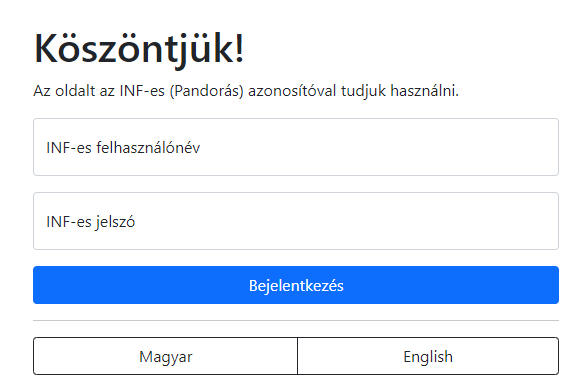
\includegraphics[width=0.6\textwidth]{userguide/main-page}
	\caption{Főoldal}
	\label{fig:main-page}
\end{figure}
\subsection{Bejelentkezés}
A rendszerbe bejelentkezni az INF-es felhasználónkkal tudunk. Ha a bejelentkezés sikertelen volt, azt a rendszer hibaüzenetekkel jelzi a számunkra (\ref{fig:login-error} ábra). 
\begin{figure}[H]
	\centering
	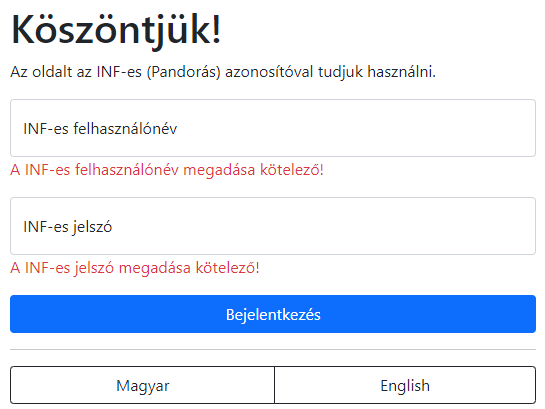
\includegraphics[width=0.6\textwidth]{userguide/login-error}
	\caption{Bejelentkezési hiba}
	\label{fig:login-error}
\end{figure}
Amennyiben a bejelentkezés sikeres volt, a \emph{szerepkörnek} megfelelő kezdőoldalon találjuk magunkat (\ref{fig:logged-in} ábra).
\begin{figure}[H]
	\centering
	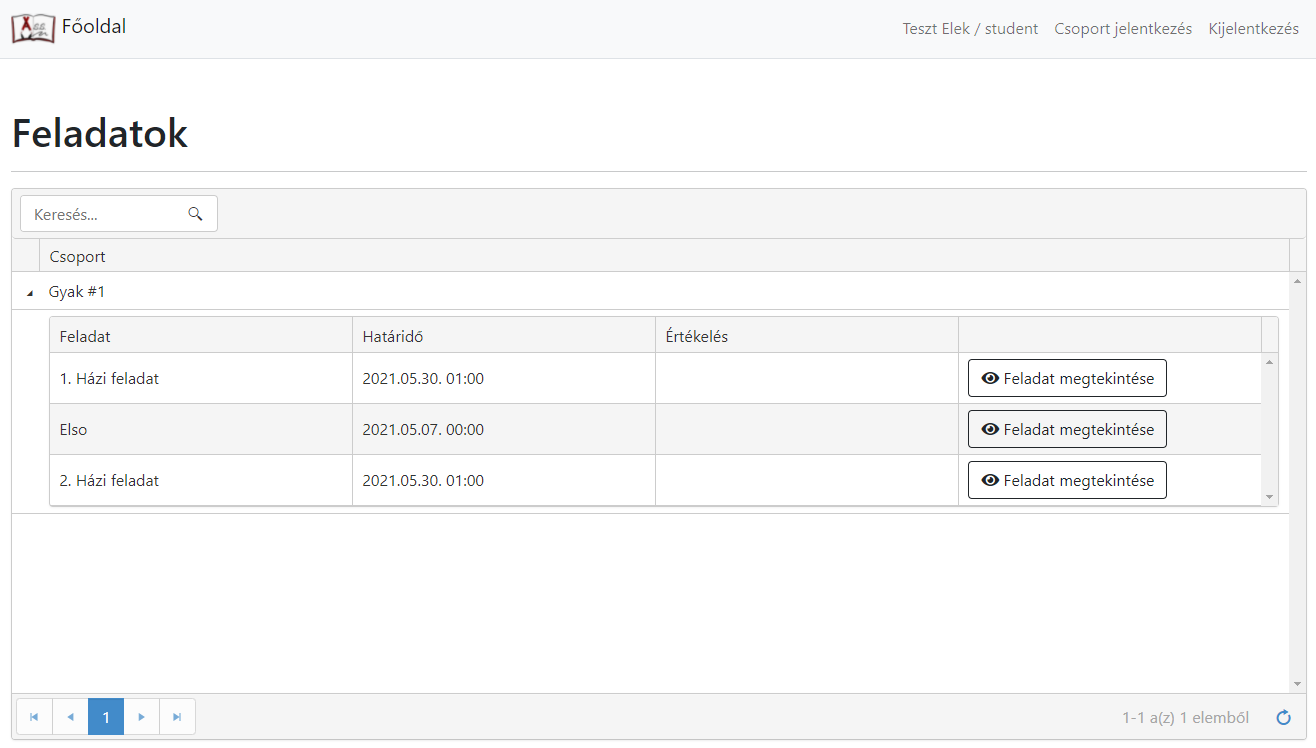
\includegraphics[width=1.0\textwidth]{userguide/logged-in}
	\caption{Sikeres bejelentkezés}
	\label{fig:logged-in}
\end{figure}
\subsection{Nyelvválasztás}
A rendszer kilistázza a támogatott lokalizációkat (jelenleg magyar és angol). Alapértelmezett beállítás a magyar. Ezt felültudjuk írni, ha valamelyik gombra rákattintunk. (\ref{fig:change-lang} ábra)
\begin{figure}[H]
	\centering
	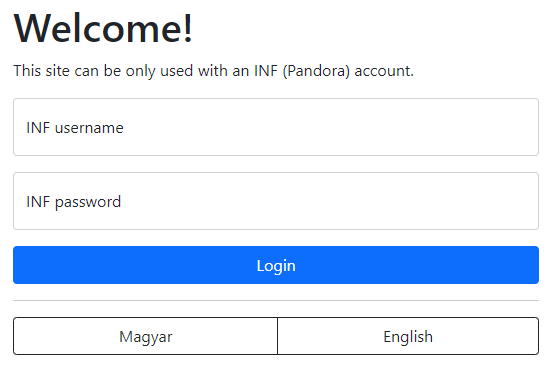
\includegraphics[width=0.6\textwidth]{userguide/change-lang}
	\caption{Nyelvváltás}
	\label{fig:change-lang}
\end{figure}
\section{Szerepkörök}
A felhasználók négy csoportba tartozhatnak:
\begin{compactitem}
    \item \hyperref[step:admin-role]{Rendszergazda}
    \item \hyperref[step:teacher-role]{Tárgyfelelős}
    \item \hyperref[step:instructor-role]{Gyakorlatvezető}
    \item \hyperref[step:student-role]{Hallgató}
\end{compactitem}
Egy felhasználó tartozhat több szerepkörbe. Ha egy felhasználó több szerepkörbe is tartozik, akkor a felület menüsorán megjelenik egy "Szerepkör váltás" lenyitható menü, ahol a felhasználóhoz rendelt szerepköröket találjuk, a kiválasztott linkre kattintva a csoporthoz tartozó kezdőoldalra navigáljuk magunkat. A felhasználóhoz a szerepköröket a felhasználó létrehozásakor is megadhatjuk, valamint a létrehozást követően tudjuk módosítani.
\subsection{Rendszergazda}\label{step:admin-role}
A rendszergazda a következő funkciókat érheti el:
\begin{compactitem}
    \item Tantárgy létrehozása, módosítása, törlése, tárgyi információk megtekintése
    \item Felhasználó létrehozása, módosítása, a felhasználók adatainak a megtekintése
\end{compactitem}
Ha rendszergazdaként jelentkezünk be az alábbi két táblázat fogad minket a kezdőoldalon~(\ref{fig:admin-page} ábra). 
\begin{figure}[H]
	\centering
	\subfigure[Tantárgyak táblázata]{
		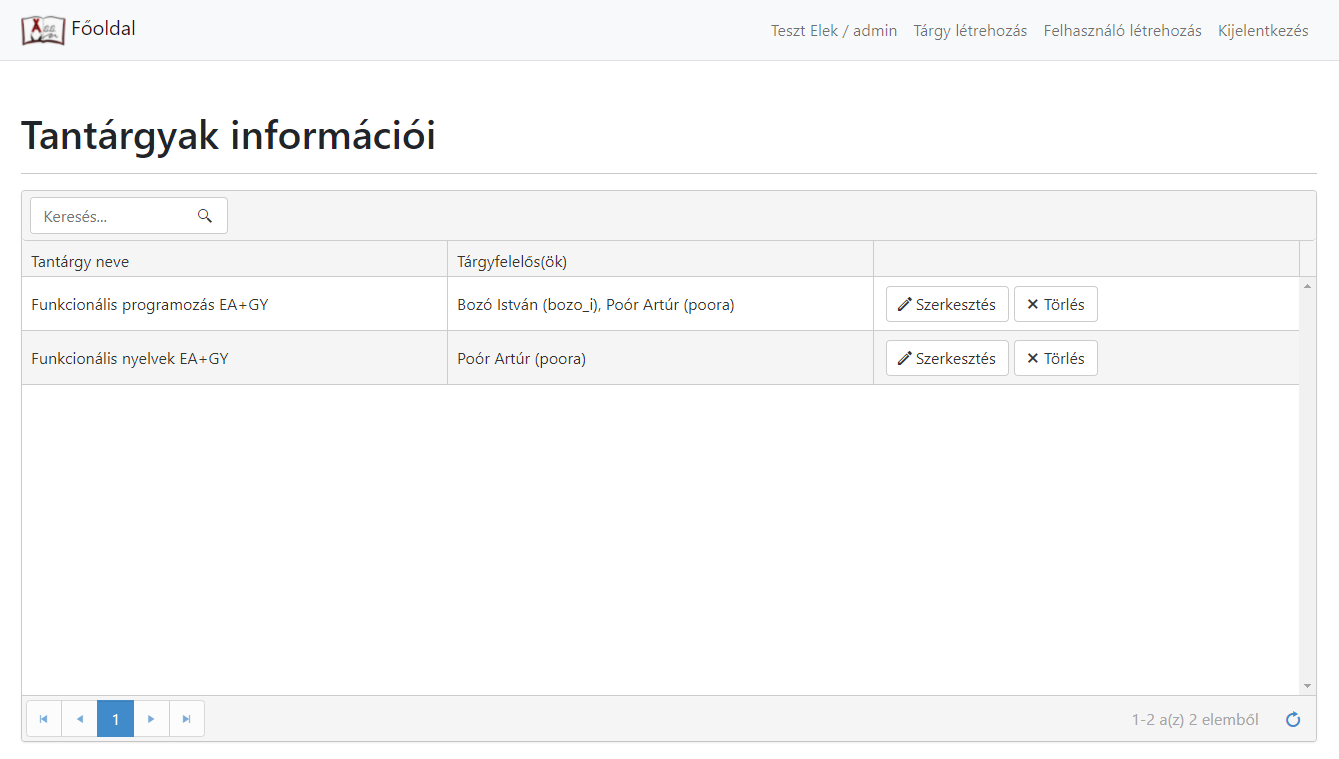
\includegraphics[width=1\linewidth]{userguide/admin-table1}
        \label{subfig:admin-subject-table}}
	\hspace{5pt}
	\subfigure[Felhasználók táblázata]{
		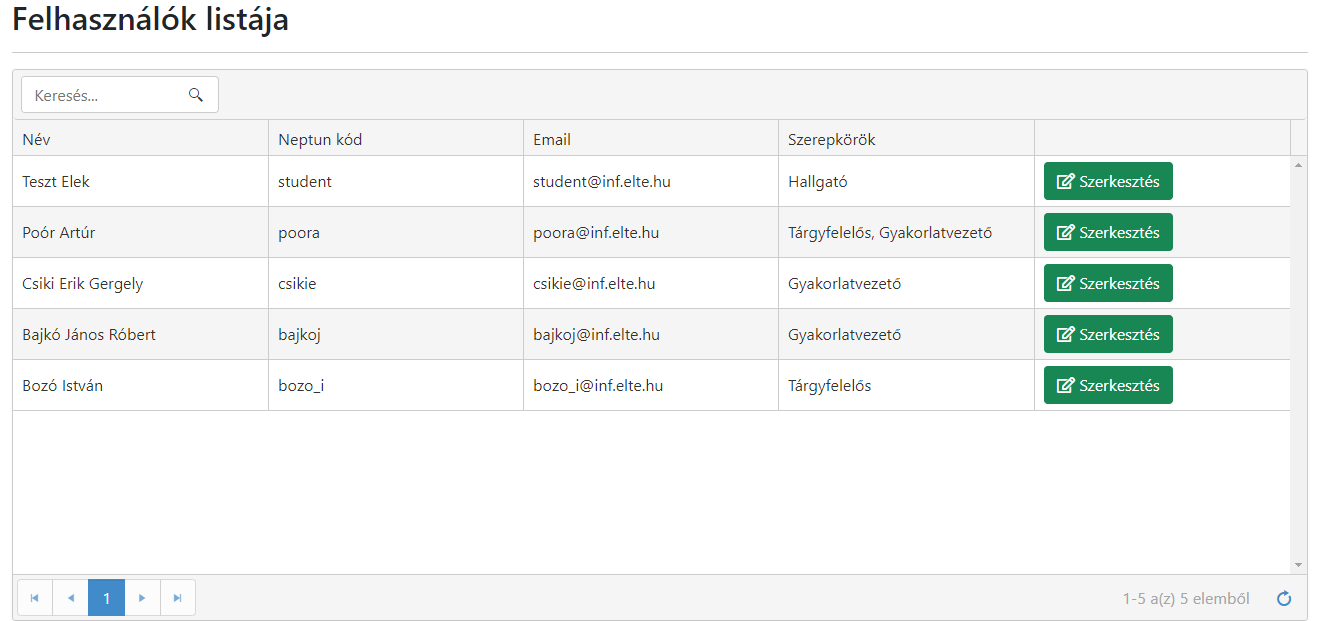
\includegraphics[width=1\linewidth]{userguide/admin-table2}
        \label{subfig:admin-users-table}}
	\caption{Rendszergazdai szerepkör kezdőoldala}
	\label{fig:admin-page}
\end{figure}
Az első táblázatban a rendszerben létrehozott tantárgyak és a hozzájuk tartozó információk olvashatóak le. A táblázatban az egyes tantárgyakhoz tartozó adatok módosíthatóak, illetve az egész tárgyat lehet törölni. A módosítás során validálásra kerül, hogy a módosított név létezik-e már a rendszerben, ha igen, akkor ezt a rendszer jelzi számunkra. A második táblázatban a rendszerben létrehozott felhasználókat és a hozzájuk tartozó információkat láthatjuk. A rendszergazda a felhasználók adatait és szerepköreit tudja módosítani.
\subsubsection{Tantárgy létrehozása}
A ``Tárgy létrehozás'' linkre kattintva az alkalmazás átnavigál minket egy űrlapra, ahol az új tantárgy szükséges adatait tudjuk kitölteni (\ref{subfig:admin-create-subject} ábra). Ha az adatok validálása és feldolgozása sikeres, akkor visszanavigálódunk a kezdőoldalra. Az esetleges validalási hibákat a rendszer jelzi számukra (\ref{subfig:admin-create-subject-error} ábra).
\begin{figure}[H]
	\centering
	\subfigure[Űrlap]{
		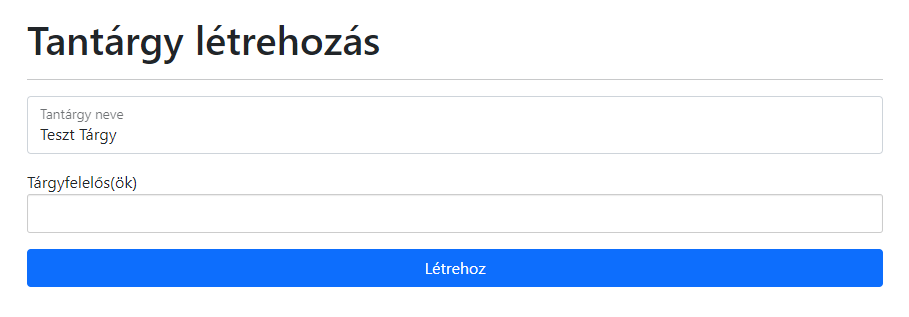
\includegraphics[width=0.8\linewidth]{userguide/admin-create-subject-form}
        \label{subfig:admin-create-subject}}
	\hspace{5pt}
	\subfigure[Adatok validálása]{
		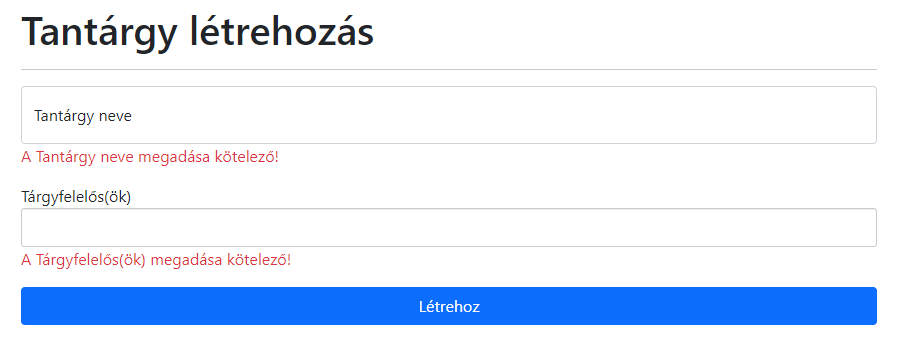
\includegraphics[width=0.8\linewidth]{userguide/admin-create-subject-error}
        \label{subfig:admin-create-subject-error}}
	\caption{Tantárgy létrehozás}
	\label{fig:admin-create-subject}
\end{figure}
\subsubsection{Felhasználó létrehozása}
Felhasználót létrehozni a ``Felhasználó létrehozás'' linkre kattintva tudjuk megtenni, ami továbbnavigál minket egy űrlapra, ahol az új felhasználónak az adatait tudjuk megadni (\ref{subfig:admin-create-user} ábra). Ha az adatok validálása sikeres, akkor a felhasználó elkészült és visszanavigálódunk a kezdőoldalra, ha nem volt sikeres, akkor a rendszer ezt hibaüzenetekkel jelzi nekünk (\ref{subfig:admin-create-user-error} ábra).
\begin{figure}[H]
	\centering
	\subfigure[Űrlap]{
		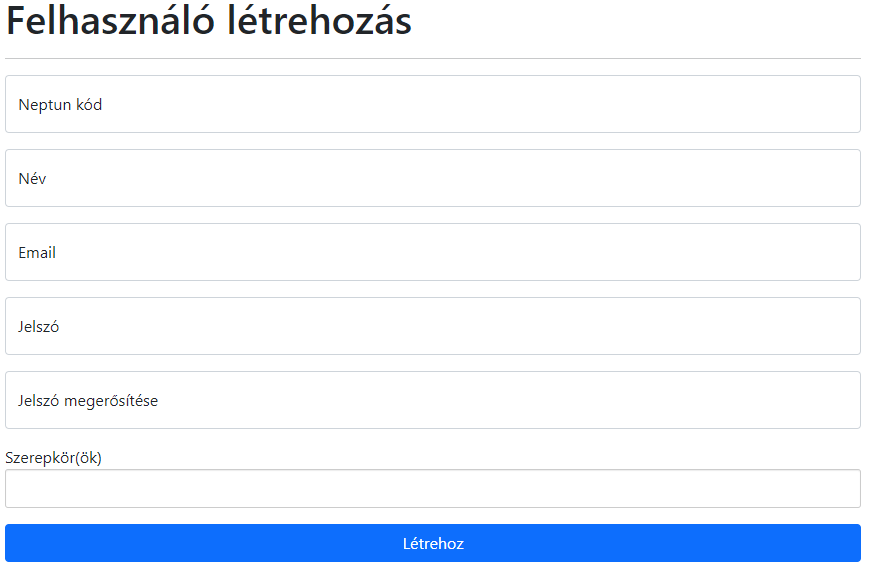
\includegraphics[width=0.7\linewidth]{userguide/admin-create-user-form}
        \label{subfig:admin-create-user}}
	\hspace{5pt}
	\subfigure[Adatok validálása]{
		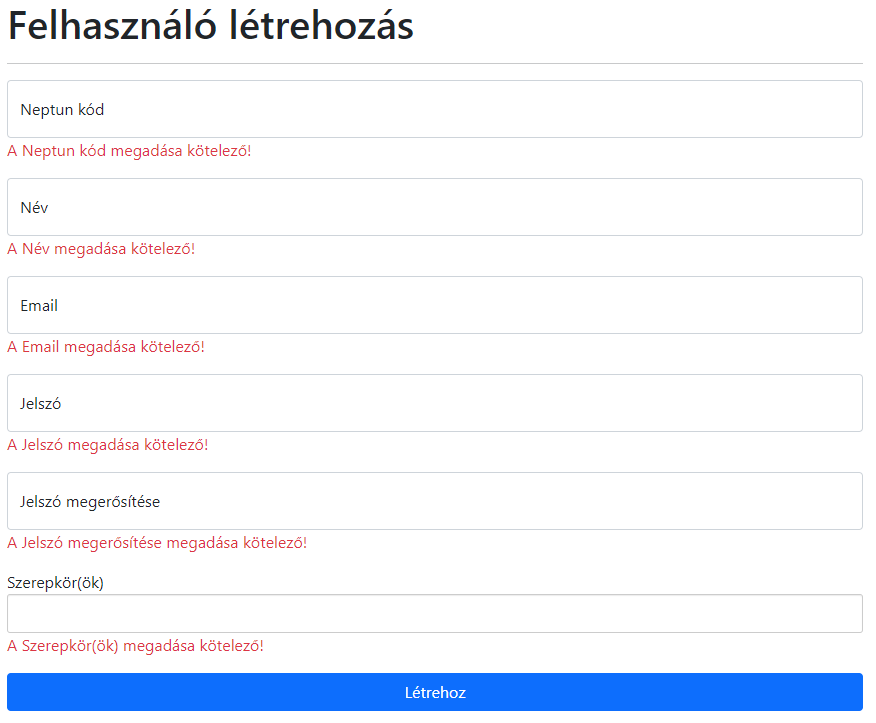
\includegraphics[width=0.85\linewidth]{userguide/admin-create-user-error}
        \label{subfig:admin-create-user-error}}
	\caption{Felhasználó létrehozás}
	\label{fig:admin-create-user}
\end{figure}
\subsection{Tárgyfelelős}\label{step:teacher-role}
Ha tárgyfelelősként jelentkezünk be a rendszerbe, akkor az alábbi kezdőoldal fogad minket (\ref{fig:teacher-home} ábra).
A kezdőoldalon egy táblázat található, amiben látjuk azokat a tantárgyakat, és a tantárgyakhoz tartozó csoportokat, amelyeknek a felelősei vagyunk.
A tárgyfelelős a következő funkciókat használhatja:
\begin{compactitem}
    \item \hyperref[step:teacher-create-course]{Csoport létrehozása egy tantárgyhoz}
    \item \hyperref[step:teacher-edit-course]{Csoport módosítása}
\end{compactitem}
\begin{figure}[H]
	\centering
	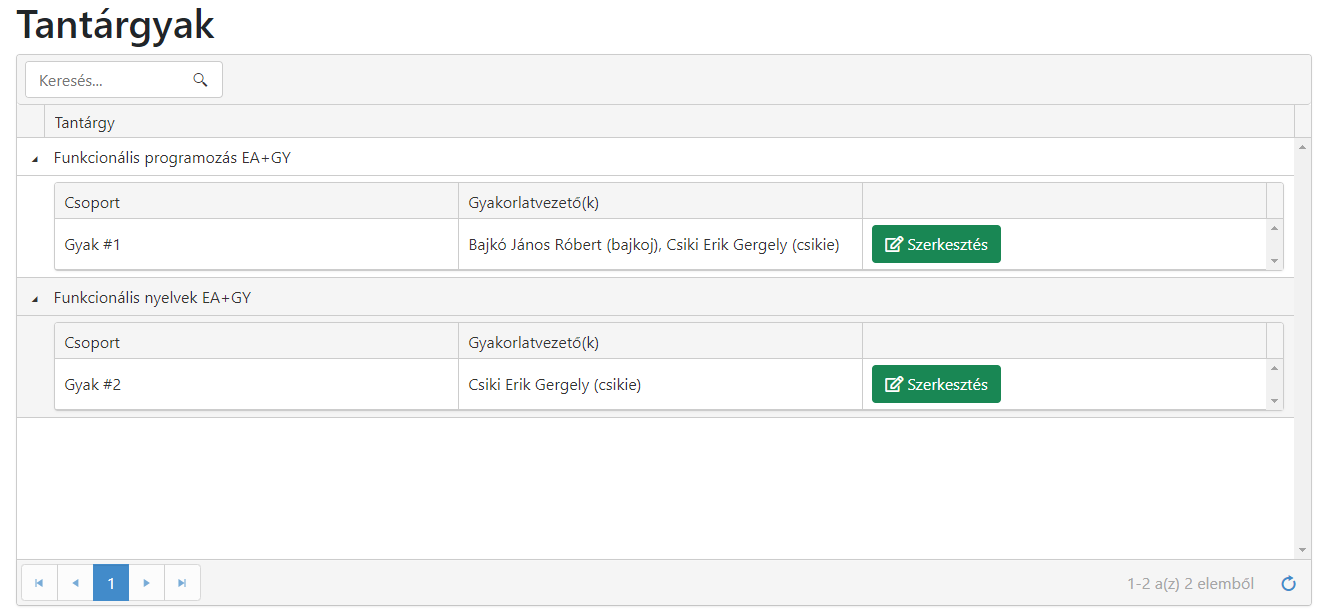
\includegraphics[width=1.0\textwidth]{userguide/teacher-home}
	\caption{Tárgyfelelős kezdőoldala}
	\label{fig:teacher-home}
\end{figure}
\subsubsection{Csoport létrehozása}
\label{step:teacher-create-course}
A menüsoron a ``Csoport létrehozás'' linkre kattintva a rendszer átirányít minket egy űrlapra, ahol létre tudunk hozni egy csoportot (\ref{fig:teacher-create-course} ábra). Az adatokat a rendszer validálja, és az esetleges hibákat jelzi számunkra.
\begin{figure}[H]
	\centering
	\subfigure[Űrlap]{
		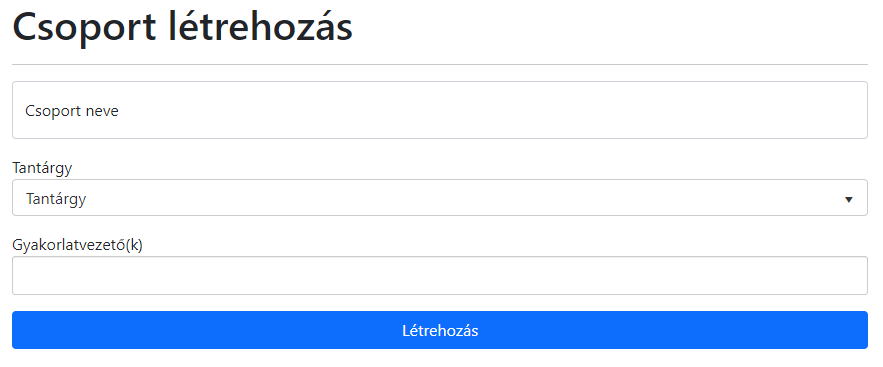
\includegraphics[width=0.75\linewidth]{userguide/teacher-create-course-form}
        \label{subfig:teacher-create-course-form}}
	\hspace{5pt}
	\subfigure[Adatok validálása]{
		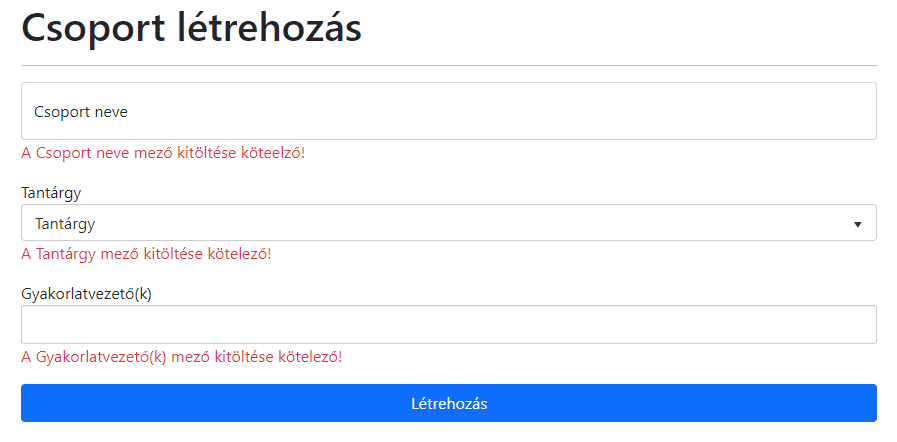
\includegraphics[width=0.75\linewidth]{userguide/teacher-create-course-error}
        \label{subfig:teacher-create-course-error}}
	\caption{Csoport létrehozás}
	\label{fig:teacher-create-course}
\end{figure}
\subsubsection{Csoport módosítása}
\label{step:teacher-edit-course}
Csoportokat szerkeszteni a kezdőoldalon található táblázat segítségével tudunk. A táblázatban lenyitható minden kilistázott tantárgy. Itt találjuk a tantárgyakhoz már létrehozott csoportokat. Minden tantárgy mellett találunk egy ``Szerkesztés'' gombot, melyre kattintva elérhetővé válik a csoport szerkesztése. Az adatok validálásra kerülnek, az esetleges hibákat a rendszer jelzi számunkra (\ref{fig:teacher-edit-course} ábra).
\begin{figure}[H]
	\centering
	\subfigure[Űrlap]{
		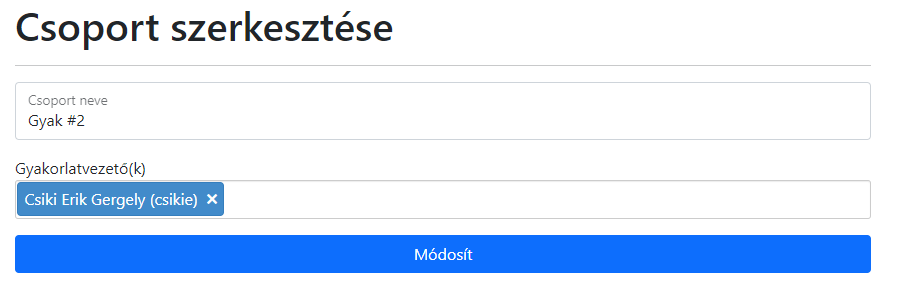
\includegraphics[width=0.75\linewidth]{userguide/teacher-edit-course-form}
        \label{subfig:teacher-edit-course-form}}
	\hspace{5pt}
	\subfigure[Adatok validálása]{
		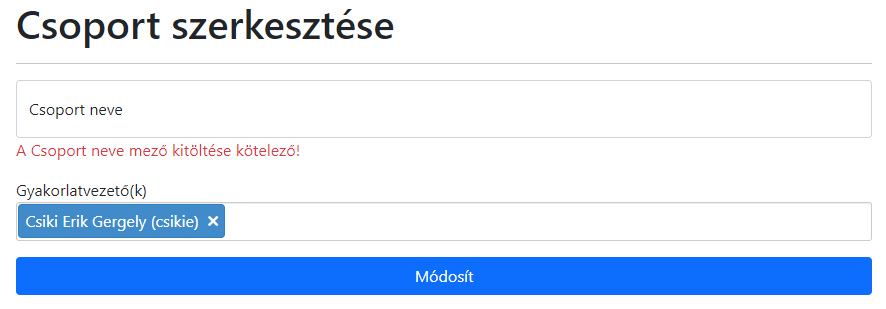
\includegraphics[width=0.75\linewidth]{userguide/teacher-edit-course-error}
        \label{subfig:teacher-edit-course-error}}
	\caption{Csoport módosítása}
	\label{fig:teacher-edit-course}
\end{figure}
\subsection{Gyakorlatvezető}\label{step:instructor-role}
Gyakorlatvezetőként bejelentkezve a rendszerbe a \ref{fig:instructor-home} ábrán látható kezdőoldal fogad minket. Az oldalon az ``Értékelendő beadandók'' cím alatt, a hozzánk rendelt csoportok hallgatóit láthatjuk egy-egy táblázatban, ahol láthatjuk, hogy egy hallgató az adott feladatra adott-e be megoldást. A ``Hallgatói várólista'' cím alatt szintén egy táblázatot találunk (\ref{subfig:instructor-table2} ábra), ahol tantárgyanként csoportosítva a következő információkat olvashatjuk le:
\begin{compactitem}
    \item Hallgató neve
	\item Hallgató neptun kódja
	\item Csoport neve
\end{compactitem}
\begin{figure}[H]
	\centering
	\subfigure[Értékelendő beadandók]{
		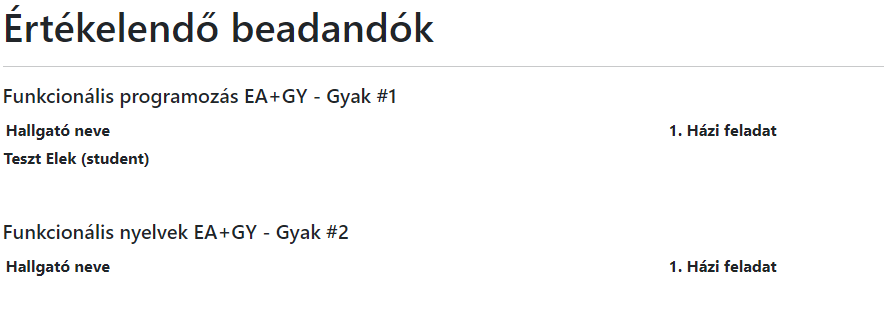
\includegraphics[width=0.75\linewidth]{userguide/instructor-table1}
        \label{subfig:instructor-table1}}
	\hspace{5pt}
	\subfigure[Hallgatói várólista]{
		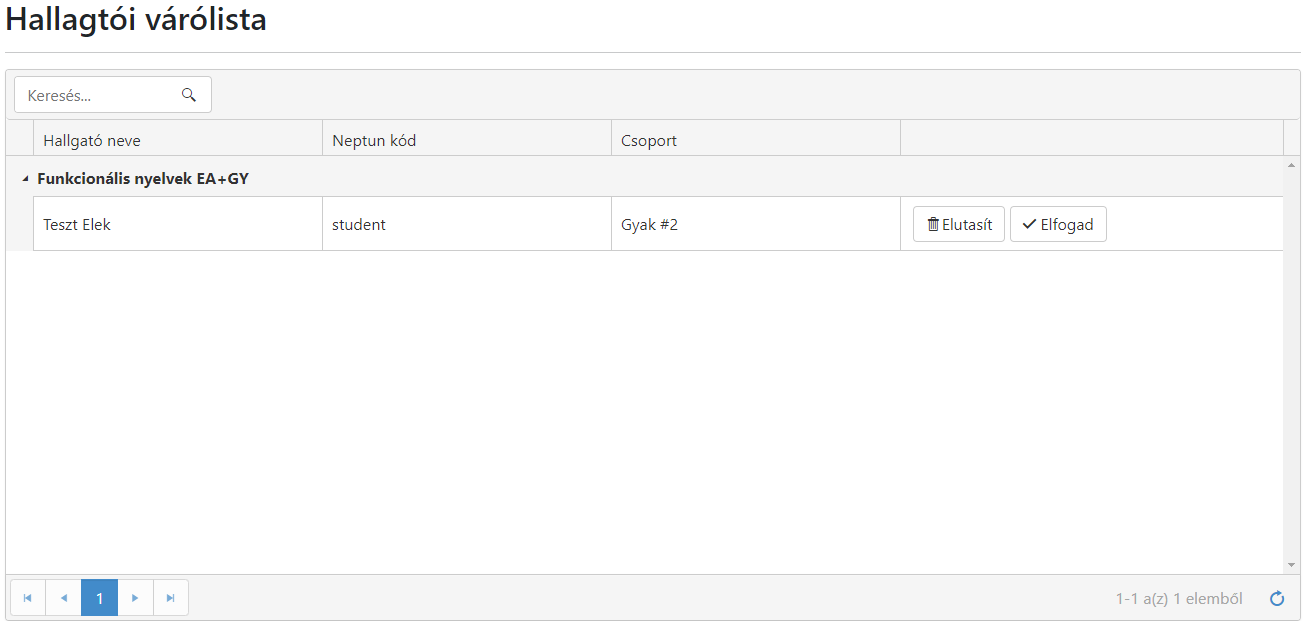
\includegraphics[width=1\linewidth]{userguide/instructor-table2}
        \label{subfig:instructor-table2}}
	\caption{Gyakorlatvezető kezdőoldala}
	\label{fig:instructor-home}
\end{figure}
A gyakorlatvezető az alábbi funkciókat éri el:
\begin{compactitem}
    \item \hyperref[step:instructor-create-assignment]{Feladat kiírása}
	\item \hyperref[step:instructor-pending]{Jelentkezések bírálata}
	\item \hyperref[step:instructor-eval]{Beadott munka értékelése}
\end{compactitem}
\subsubsection{Feladat kiírása}
\label{step:instructor-create-assignment}
Feladatot kiírni a ``Feladat létrehozása'' menüpont alatt tudunk, ahol egy űrlapot találunk (\ref{fig:instructor-create-assignment}). Ahhoz hogy létrehozzunk egy feladatot, a következő információkat szükséges megadnunk:
\begin{compactitem}
    \item A feladat neve
    \item Kezdés és befejezés dátuma
	\item Feladat leírása
	\item Mely csoporthoz legyen létrehozva\footnote{A lenyíló kiválasztó menüben lehetőségünk van több csoportot is kiválasztani}
\end{compactitem}
\begin{figure}[H]
	\centering
	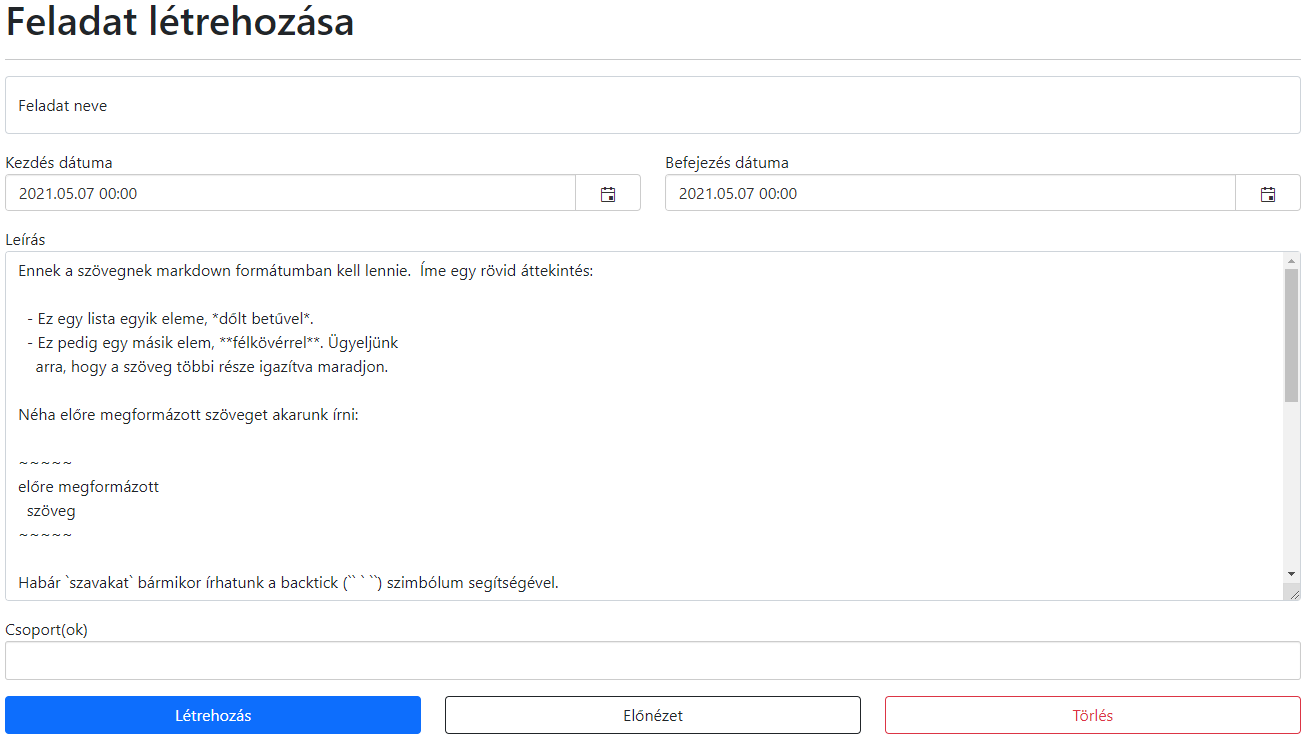
\includegraphics[width=1.0\textwidth]{userguide/instructor-create-assignment}
	\caption{Feladat létrehozás}
	\label{fig:instructor-create-assignment}
\end{figure}
A rendszer támogatja, hogy a feladatnak leírása ne csak egyszerű szöveg legyen. A szövegdobozban megadhatunk \texttt{Markdown} és \LaTeX\ kifejezéseket is. Mielőtt létrehoznánk a feladatot, meg tudjuk tekinteni, hogy a hallgató milyen formában fogja látni a kiírva a feladatot. Így le tudjuk ellenőrizni kényelmesen a feladat leírását, valamint azt is tudjuk ellenőrizni, hogy a \texttt{Markdown} és \LaTeX\ kifejezéseinket helyesen írtuk-e meg. Ha végeztünk, a ``Létrehozás'' gombbal tudjuk elküldeni a rendszernek az adatokat. Az adatokat a rendszer leellenőrzi, az esetleges hibákat jelzi számunkra (\ref{fig:instructor-create-assignment-error}).
\begin{figure}[H]
	\centering
	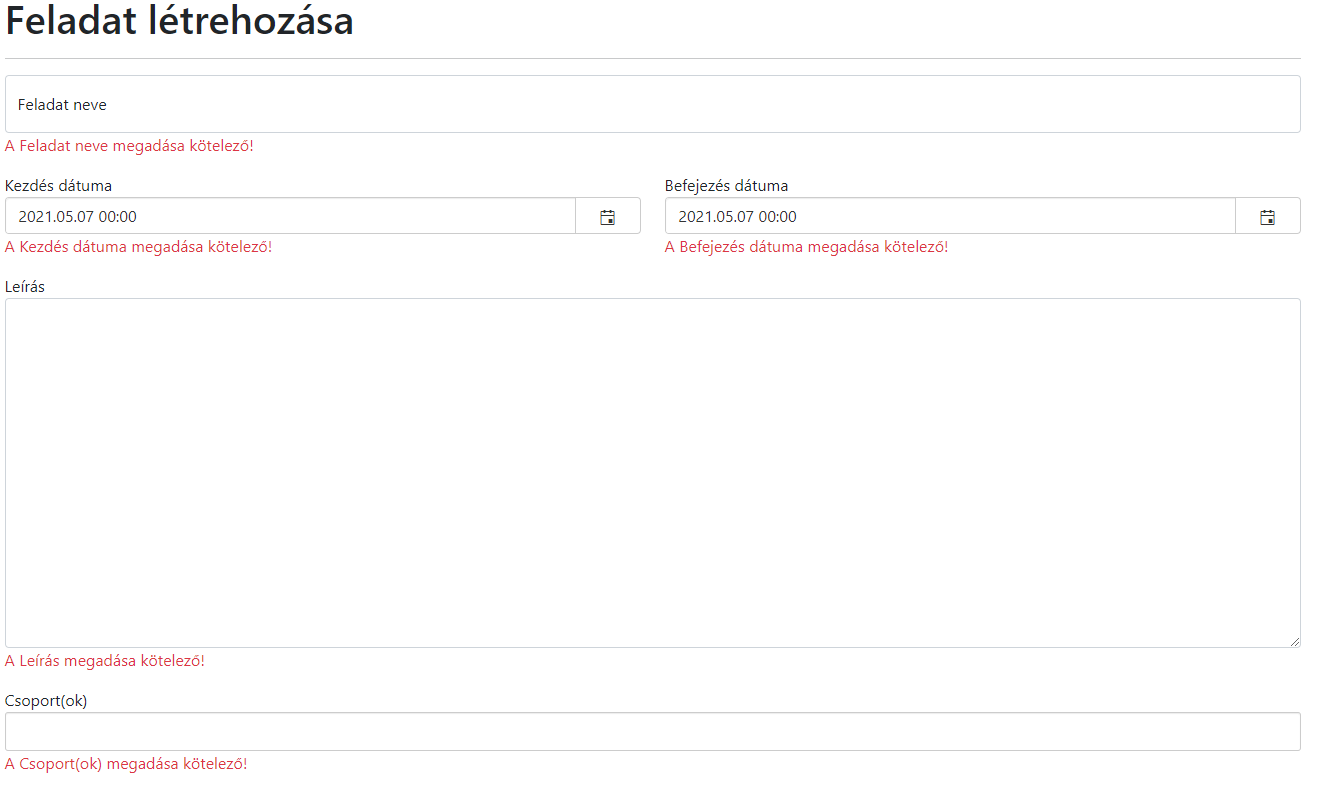
\includegraphics[width=1.0\textwidth]{userguide/instructor-create-assignment-error}
	\caption{Adatok validálása}
	\label{fig:instructor-create-assignment-error}
\end{figure}
\subsubsection{Jelentkezések bírálata}
\label{step:instructor-pending}
Egy hallgatónak a csoportba való jelentkezését a ``Hallgatói várólista'' táblázatában tudjuk megtenni (\ref{subfig:instructor-table2} ábra), az utolsó oszlopban lévő gombok segítségével. Miután elvégeztük a bírálatot, a táblázatból törlődik a jelentkezett hallgató, és az oldal frissítése után, a megfelelő táblázatban látjuk, hogy a hallgatót a rendszer felvette a jelentkezett csoportba.
\subsubsection{Beadott munka értékelése}
\label{step:instructor-eval}
Egy feladatra beadott megoldás értékeléséhez a kívánt feladat oszlopában kattintsunk a \emph{szürke négyzetre}. Ilyenkor a rendszer átirányít minket az értékelő felületre (\ref{fig:instructor-eval-assignment}). A rendszer a felületre a ``Megoldás(ok)'' alatt felsorolja a hallgatónak az összes beadott megoldását a beküldés ideje szerint csökkenően rendezve. Elég egy megoldást értékelnünk, de értékelhetjük az összeset is. Viszont a rendszer a legutolsó értékelést veszi számításba. Ezt fogja a hallgató is látni. A beadott megoldások között a kívánt sorra kattintva tudjuk kiválasztani, hogy melyik megoldást szeretnénk változtatni. Ilyenkor a ``Beadott megoldás'' alatt látjuk, mi a hallgatónak a beadott megoldása. Az értékelésünket az oldal alján található űrlapon tudjuk megtenni. Az értékelés után a rendszer a kezdőoldalra navigál minket. Az értékelt feladatnál a \emph{szürke négyzet} egy \emph{körben lévő pipára} cserélődik.
\begin{figure}[H]
	\centering
	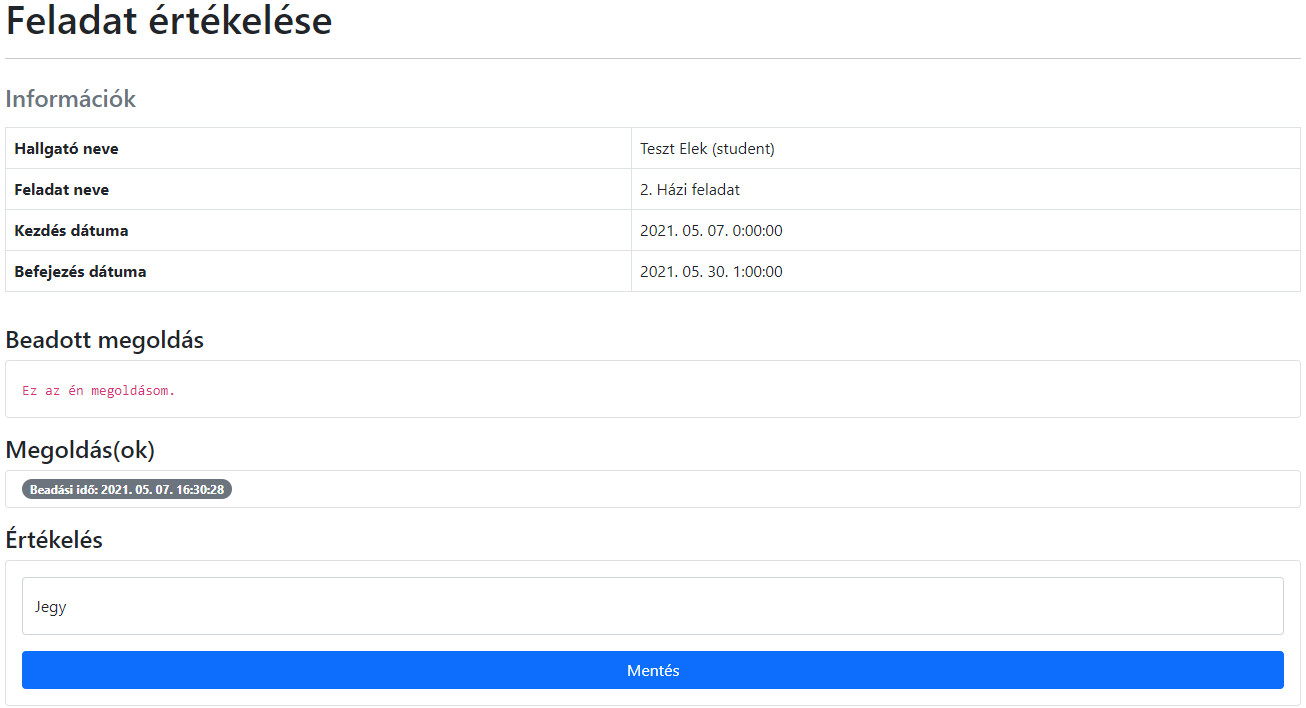
\includegraphics[width=1.0\textwidth]{userguide/instructor-eval-assignment}
	\caption{Feladat értékelése}
	\label{fig:instructor-eval-assignment}
\end{figure}
\subsection{Hallgató}
\label{step:student-role}
Hallgatóként bejelentkezve a \ref{fig:student-home} ábrán látható kezdőoldal fogad minket. A ``Feladatok'' cím alatti táblázatban a hallgató számára listázásra kerül az összes olyan csoportja, ahova elfogadták a jelentkezését. A táblázatban csoportokra lebontva jelennek meg a hallgató számára a kiírt feladatok. A táblázatban egy feladatról a következő információkat láthatjuk: neve, határideje, kapott értékelés.
\begin{figure}[H]
	\centering
	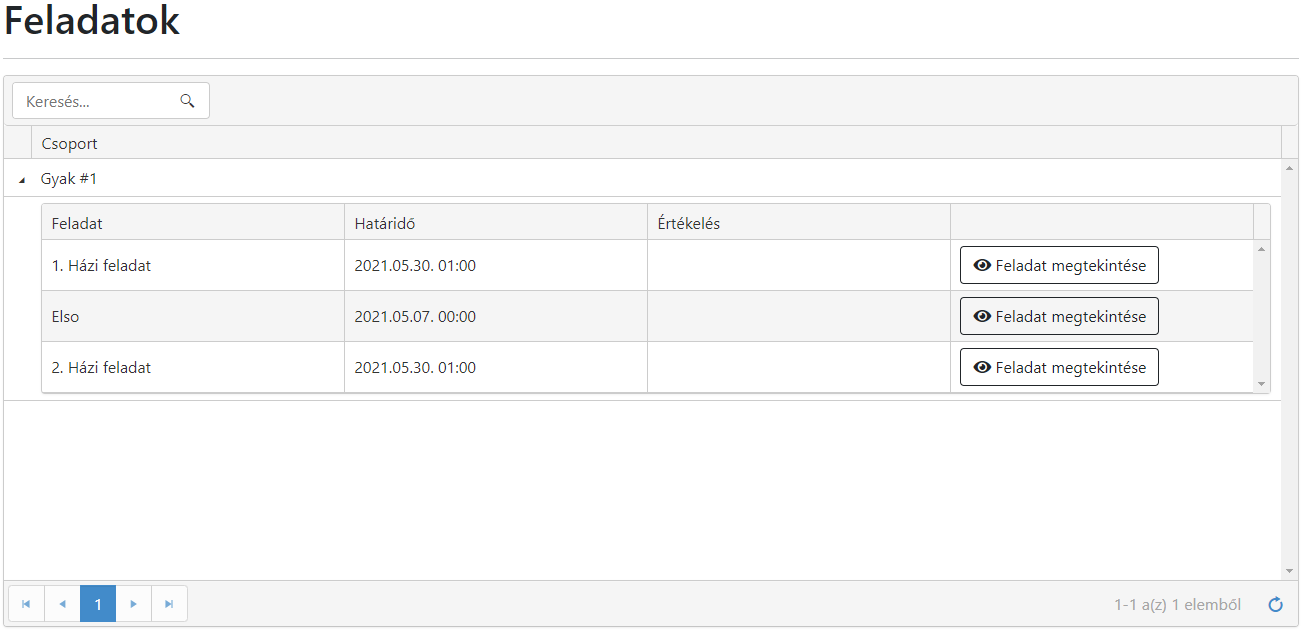
\includegraphics[width=1.0\textwidth]{userguide/student-home}
	\caption{Hallgató kezdőoldala}
	\label{fig:student-home}
\end{figure}
A hallgató az alábbi funkciókat használhatja:
\begin{compactitem}
    \item \hyperref[step:student-course-reg]{Csoportba jelentkezés}
	\item \hyperref[step:student-solution]{Megoldás beadása}
\end{compactitem}
\subsubsection{Csoportba jelentkezés}
\label{step:student-course-reg}
Csoportba jelentkezni a ``Csoport jelentkezés'' menüpontra kattintva tudunk. A rendszer egy űrlapot biztosít számunkra (\ref{fig:student-course-reg} ábra), ahol listázásra kerülnek a rendszerben található csoportok, amelyekre még nem jelentkeztünk. A rendszer lehetőséget biztosít számunkra, hogy akár egyszerre több csoportra is leadjuk a jelentkezésünket. Jelentkezésünket a ``Jelentkezés'' gombbal tudjuk továbbítani a rendszer számára. Az űrlap validálásra kerül, hogy üresen ne tudjuk beküldeni azt. Sikeres jelentkezés esetén a rendszer a kezdőoldalra navigál minket.
\begin{figure}[H]
	\centering
	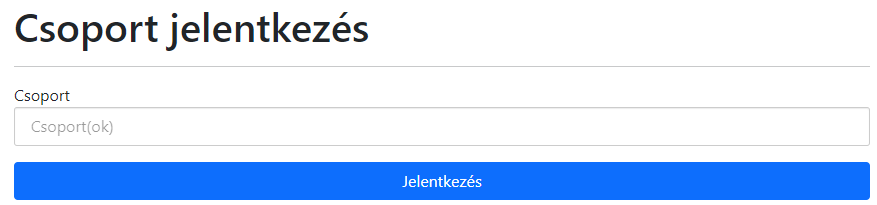
\includegraphics[width=1.0\textwidth]{userguide/student-course-reg}
	\caption{Csoportba jelentkezése}
	\label{fig:student-course-reg}
\end{figure}
\subsubsection{Megoldás beadása}
\label{step:student-solution}
Megoldás beküldéséhez válasszuk ki a kívánt feladatot, amire megoldást szeretnénk beküldeni, majd kattintsunk a ``Feladat megtekintése'' gombra. Ekkor a rendszer egy új ablakban megnyitja a feladatot (\ref{fig:student-submit-sol} ábra). Az oldalon a következő információkat látjuk:
\begin{compactitem}
    \item Határidő visszaszámláló
    \item Feladat neve, leírása
    \item Beküldött megoldások
    \item Űrlap a megoldás beküldéséhez
\end{compactitem}
\begin{figure}[H]
	\centering
	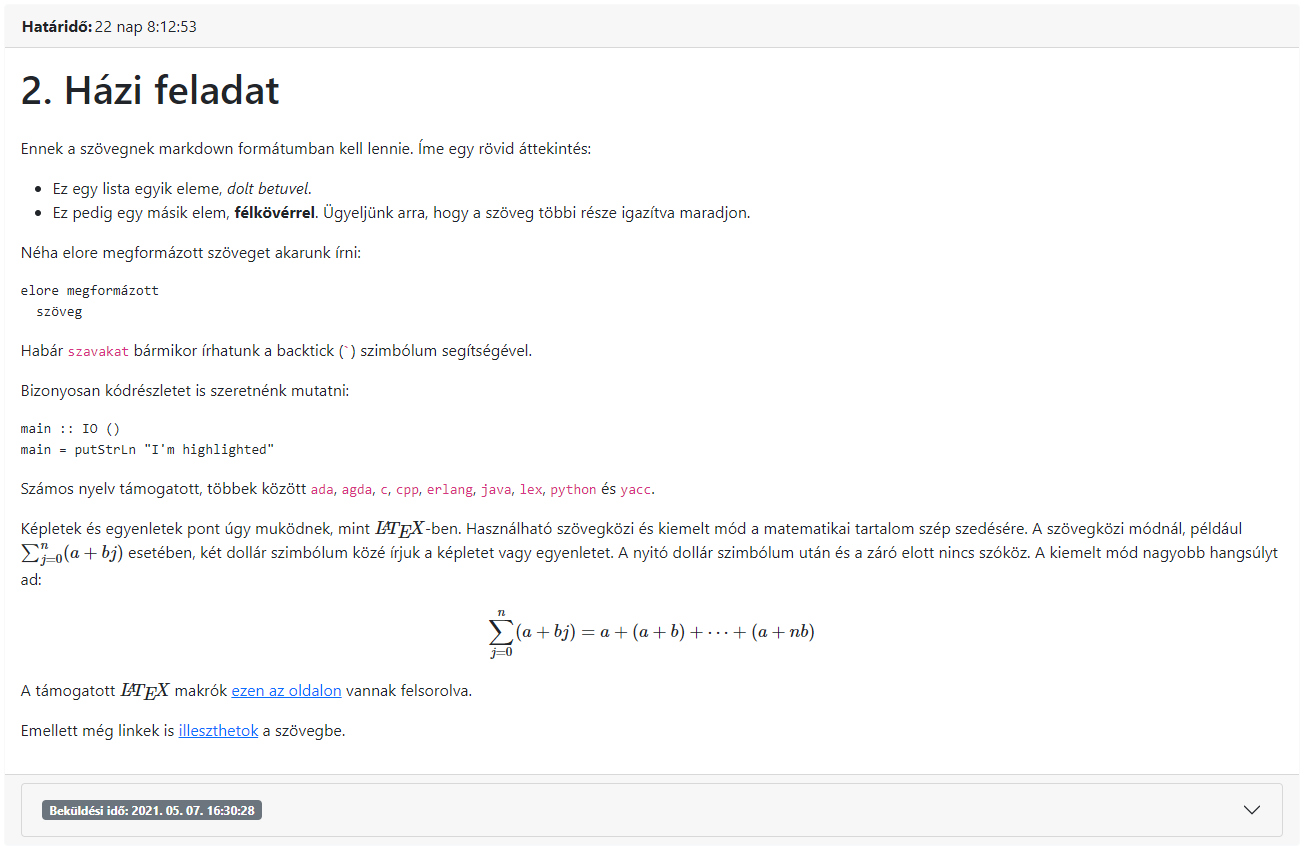
\includegraphics[width=1.0\textwidth]{userguide/student-submit-sol}
	\caption{Feladat megtekintése}
	\label{fig:student-submit-sol}
\end{figure}
\subsection{Mindenki számára elérhető oldalak}
\label{step:mindenkinek-elerheto-oldal}
A rendszerben jelenleg három olyan oldal található, amelyet minden szerepkörben elérhetünk. Az egyik oldal a felhasználónk adatainak megtekintésére szolgál. Ezt a funkciót a menüsoron a nevünkre kattintva tudjuk elérni. Ezen a felületen (\ref{fig:profile} ábra) a következőket tekinthetjük meg a ``Személyes adatok'' cím alatt: név, neptun kód, e-mail cím és a felhasználónkhoz rendelt szerepkörök. Ezen felületen továbbá be tudjuk állítani, hogy a rendszer milyen lokalizációval működjön (magyar és angol). Ezt a megfelelő gombra kattintva tudjuk változtatni.
\begin{figure}[H]
	\centering
	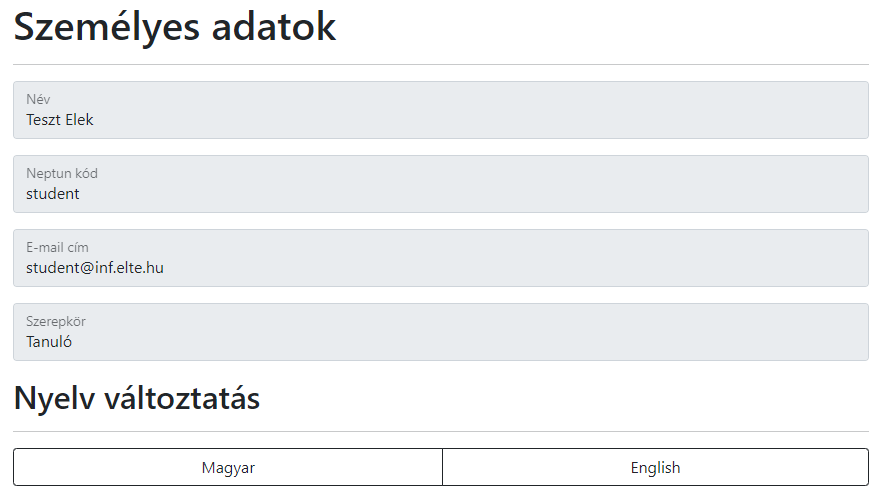
\includegraphics[width=0.8\textwidth]{userguide/profil}
	\caption{Profil oldal}
	\label{fig:profile}
\end{figure}
A másik két oldal az esetleges nem várt hibákról tájékoztat minket. Ezen hibák két kategóriába oszthatók: jogosulatlan kérés a rendszer felé, egyéb nem várt hiba. Jogosulatlan kérés akkor lép fel, ha megpróbálunk a szerepkörünkhöz nem tartozó funkciót elérni a rendszerben. Például: csak hallgatói szerepkörrel rendelkező felhasználóval vagyunk bejelentkezve a rendszerbe és a webcím végén a ``Student''-et lecseréljük ``Admin''-ra. Ezzel olyan kérést indítunk a rendszernek, hogy navigáljon minket a rendszergazdai szerepkörhöz tartozó kezdőoldalra, amihez nincs jogosultságunk, ezért a rendszer megtagadja a hozzáférést a kért oldalhoz. Ilyenkor a rendszer az alábbi \ref{fig:access-denied} ábrán látható oldalra navigál minket, ahonnan lehetőségünk van visszatérni a szerepkörünkhöz tartozó kezdőoldalra.
\begin{figure}[H]
	\centering
	
\includegraphics[width=1.0\textwidth]{userguide/access-denied}
	\caption{Jogosulatlan kérés}
	\label{fig:access-denied}
\end{figure}
Egyéb nem várt hiba lehet például, hogy a rendszer nem tud csatlakozni a hozzá tartozó adatbázishoz. Ilyenkor az alábbi \ref{fig:errors} ábrán látható oldalra navigál minket.
\begin{figure}[H]
	\centering
	
\includegraphics[width=1.0\textwidth]{userguide/errors}
	\caption{Egyéb nem várt hiba}
	\label{fig:errors}
\end{figure}
\cleardoublepage

\chapter{Fejlesztői dokumentáció} % Developer guide
\label{ch:developer}

\section{Keretrendszerek és az alkalmazás felépítése}
\label{sec:framework-app}
\subsection{Keretrendszerek}
\label{subsec:framework}
Az alkalmazás ASP.NET core 3.1 keretrendszerben készült \cite{ASPDOTNETCORE3_1}, ami egy nyílt forráskódú, webes alkalmazások készítésére szolgáló programkönyvtár, melyet a \emph{Microsoft} fejleszt. A keretrendszer lehetővé teszi, hogy az alkalmazás több platformon is tudjon futni (\emph{Linux}, \emph{macOS} és \emph{Windows}). Továbbá a \emph{Kendo UI Core for jQuery}\cite{KendoUIforJquery} keretrendszer biztosítja számunkra a felületen található felhasználóbarát táblázatokat, űrlap elemeket. A saját \emph{HTML} elemek stílusait a \emph{Bootstrap}\cite{Bootstrap} keretrendszer biztosítja.
\subsection{Az alkalmazás felépítése}
\label{subsec:app} 
Az alkalmazás az \emph{MVC} architektúrára épül (\ref{fig:mvc-pattern} ábra)\cite{MVC}. Tehát három rétegre bontható a felépítése, Modell-Nézet-Vezérlő. A Modell (angolul \emph{Model}) réteg tartalmazza az üzleti logikát, amely az adatokat kezeli és kapcsolatban van az adatbázissal. A nézet réteg (angolul \emph{View}) felelős a megjelenítésért. A vezérlő réteg (angolul \emph{Controller}) fogadja a kliens kéréseit és válaszol azokra. Az \emph{MVC} architektúra fő előnye, hogy jól elkülöníthetőek a rétegek, így a nézet független marad a modelltől. Ezáltal, ha szükséges, könnyedén le tudjuk cserélni az egész alkalmazás nézetét, vagy fordítva újra implementálhatjuk a modell réteg működését, anélkül hogy ez a nézeten bármi gondot okozna.
\begin{figure}[H]
	\centering
	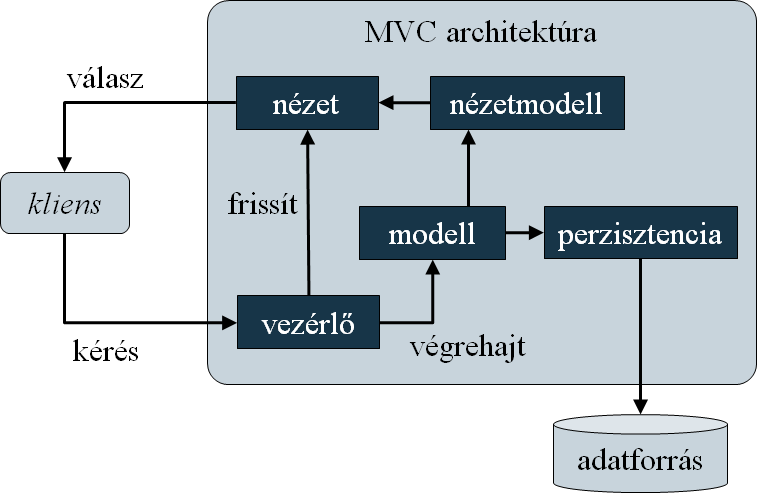
\includegraphics[width=1.0\textwidth]{developerguide/mvc-pattern}
	\caption{A Modell-Nézet-Vezérlő architektúra}
	\label{fig:mvc-pattern}
\end{figure}
Az alkalmazásban a könnyebb és egyszerűbb fejleszthetőség miatt a \emph{Model} réteget több komponensre bontjuk. Így az alábbi komponensekből áll össze a \emph{Model} réteg:
\begin{center}
	\begin{forest}
		for tree={
			font=\ttfamily,
			grow'=0,
			child anchor=west,
			parent anchor=south,
			anchor=west,
			calign=first,
			edge path={
			\noexpand\path [draw, \forestoption{edge}]
			(!u.south west) +(7.5pt,0) |- node[fill,inner sep=1.25pt] {} (.child anchor)\forestoption{edge label};
			},
			before typesetting nodes={
			if n=1
				{insert before={[,phantom]}}
				{}
			},
			fit=band,
			before computing xy={l=15pt},
		}
		[ASS
			[ASS.BLL/
				[Interfaces/]
				[Services/]
			]
			[ASS.DAL/
				[Models/]
				[ASSContext.cs]
				[DbInitializer.cs]
			]
			[ASS.WEB/
				[Models/
					[DTOs/]
					[ViewModels/]
				]
			]
		]
	\end{forest}
\end{center}
\begin{description}
	\item[ASS.BLL:]  az üzleti logikai réteget megvalósító komponens (angolul \emph{Business Logic Layer}).
	\item[ASS.DAL:] az adatelérési réteget megvalósító komponens (angolul \emph{Data Access Layer}).
	\item[ASS.WEB.Models:] ebben a komponensben tároljuk az adatok bevitelére és az adatok megjelenítésére szolgáló osztályokat.
	\item[ASSContext.cs:] az adatbázist leíró osztály.
	\item[DbInitializer.cs:] az adatbázist létrehozó statikus osztály.    
\end{description}
\section{Naplózás}
\label{sec:log}
Az alkalmazás fájl szintű naplózást tartalmaz, amit a \emph{Serilog.Extensions.Logging.File} nyílt forráskódú programkönyvtár használatával valósítjuk meg \cite{SERILOG}. Az alkalmazás automatikusan naplózza a futás közbeni eseményeket és az esetleges kivételeket. Természetesen támogatott a saját bejegyzések létrehozása is. A naplózás beállításait az \emph{appsettings.json} (\ref{src:json} ábra) fájlban tudjuk személyreszabni. Az alábbi négy értéket szabjuk személyre az alkalmazáshoz:
\begin{itemize}
	\item PathFormat: itt tudjuk megadni az alkalmazás naplófájljainak a mentési helyét, és egy sablont a fájlok nevére. A \emph{\{Date\}} paraméter helyére az aktuális dátum kerül beillesztésre (pl.: 20210513). Ha az elérési útban található mappa nem létezik azt a programkönyvtár automatikusan létrehozza a számunkra.
	\item OutputTemplate: itt adható meg a bejegyzések sablonja, hogy hogyan nézzenek ki a bejegyzés\footnote{\href{https://github.com/serilog/serilog/wiki/Formatting-Output}{Ezen a linken} részletes leírást olvashatunk az \emph{OutputTemplate}-ben használható paraméterekről.}. Az alkalmazás a következő sablont használja a bejegyzésekre: [\emph{Időbélyeg}] - [\emph{Esemény súlyossági szintje}] - [\emph{Üzenet}] \emph{Új sor} [\emph{Kivétel (ha van)}].
	\item LogLevel: itt állíthatjuk be, hogy milyen minimum szintű események kerüljenek naplózásra \cite{LogLevels}. A jelenlegi beállítással az alkalmazás minden legalább \emph{Information} szinttel rendelkező eseményt naplóz.
\end{itemize}
\newpage
\lstset{caption={Naplózás beállításai}, label=src:log}
\begin{lstlisting}[language=json]
...
"Logging": {
	"PathFormat": "../Logs/log-{Date}.log",
	"OutputTemplate": "[{Timestamp:yyyy.MM.dd HH:mm:ss}] - [{Level:u}] - {Message}{NewLine}{Exception}",
	"LogLevel": {
		"Default": "Debug",
		"Microsoft": "Information"
	}
},
...
\end{lstlisting}
\section{Adatbázis}
\label{sec:database}
\subsection{Technológiák}
Az alkalmazáshoz szükséges telepítünk egy \emph{MySQL Community Server}-re, ajánlott a \emph{8.0.25}-ös verzió.\footnote{Az alkalmazás működik régebbi verzióval is. Viszont az alkalmazás nincs felkészítve az esetleges verziók közötti különbségekre.} Az autentikáció és autorizáció megvalósításához a Microsoft által készített \emph{Microsoft.AspNetCore.Identity.EntityFrameworkCore} nyílt forráskódú programkönyvtárat használja rendszer. A programkönyvtár tartalmaz meglévő adatbázis táblákat, melyeknek a tartalma és működése elolvasható a Microsoft hivatalos honlapján \cite{Identity}. A programkönyvtár gondoskodik a jelszavak biztonságos tárolásáról, melyet időfüggő sózással és a jelszó hashelésével valósít meg.

Az adatbázis \emph{code first} módszerrel van megvalósítva, tehát nem az adatbázis szerveren \emph{SQL} kódot futattva hozzuk létre az adatbázis táblákat, hanem modell osztályokkal definiáljuk az adatbázis táblákat \cite{CodeFirst}. Ezen modelleket az \emph{ASS.DAL.Models} névtérben tároljuk.

Az adatelérést az \emph{Entity Framework Core ORM} keretrendszer biztosítja \cite{EFCore}. Az objektum-relációs leképzés (angolul \emph{Object-Relational Mapping}), egy technika az adatok konvertálására nem kompatibilis típusos rendszerek és objektumorientált programozási nyelvek között. Így az alkalmazás forráskódjában nincsenek beégetett \emph{SQL} kódok. Ezek helyett a \emph{CRUD} (Create,Read,Update,Delete műveleteknek a rövidítése) műveleteket a \emph{.NET} nyújtotta és az \emph{Entity Framework Core} által is támogatott \emph{LINQ} (Language Integrated Queries) metódushívásokkal valósul meg \cite{LINQ}. Továbbá a keretrendszer védelmet biztosít az \emph{SQL Injection} támadások ellen \cite{SQLInjection}, ugyanis a műveletek a \emph{C\#} és \emph{LINQ} metódusokból kerülnek előállításra paraméterezetten.

Az adatbázis elérését az alkalmazás konfigurációs fájljában (\emph{appsettings.json}) tudjuk megadni illetve módosítani.
\lstset{caption={Adatbázis elérése}, label=src:dbconn}
\begin{lstlisting}[language=json]
...
"ConnectionStrings": {
	"DefaultConnection": "server=localhost;database=ASS;uid=username;password=fooBarraBoof"
},
...
\end{lstlisting}
\subsection{Adatbázis \emph{code first} objektumai}
A \emph{C\#} objektumok amelyekből az adatbázis képződik a \ref{fig:daldiagram} ábrán tekinthetjük meg. Maga az adatbázis az \emph{ASSContext} osztályból képződik. Minden egyes \emph{DbSet<T>}\footnote{Ahol a \emph{T} egy generikus típusparaméter.} típusú tulajdonság (angolul Property), egy adatbázis táblát jelent. Az osztály \emph{OnModelCreating} metódusában számos adatbázisra vonatkozó beállítást van lehetőségünk beállítani (pl.: táblák elsődleges kulcsai, külső kulcsai). A \emph{DbInitializer} osztály egy nyilvános \emph{Initialize} metódussal rendelkezik, mely létrehozza az adatbázis szerveren az adatbázist, ha még nem létezik, illetve a szükséges konstans adatokkal tölti fel az adatbázist (szerepkörök felvétele és rendszergazdai felhasználó létrehozása).
\begin{figure}[H]
	\centering
	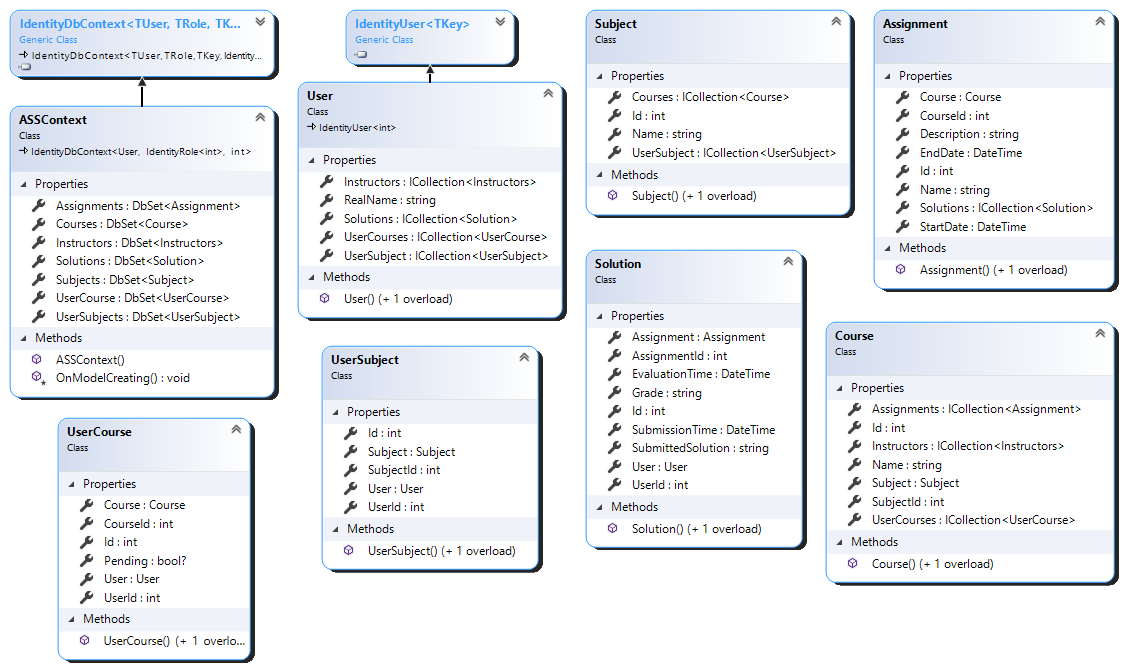
\includegraphics[width=1.0\textwidth]{developerguide/daldiagram}
	\caption{Az adatbázist leképző objektumok}
	\label{fig:daldiagram}
\end{figure}
\subsection{Az adatbázis táblái}
Az alkalmazás adatbázis diagramját a \ref{fig:dbdiagram} ábrán tekinthetjük meg. A \emph{Microsoft.AspNetCore.Identity.EntityFrameworkCore} keretrendszer által létrehozott táblákból csak azon a táblák és mezők kerülnek részletezésre, melyeket a rendszer aktívan használ. A táblák, amik nem kerülnek részletezésre a Microsoft hivatalos honlapján meg lehet tekinteni \cite{Identity}.
\begin{figure}[H]
	\centering
	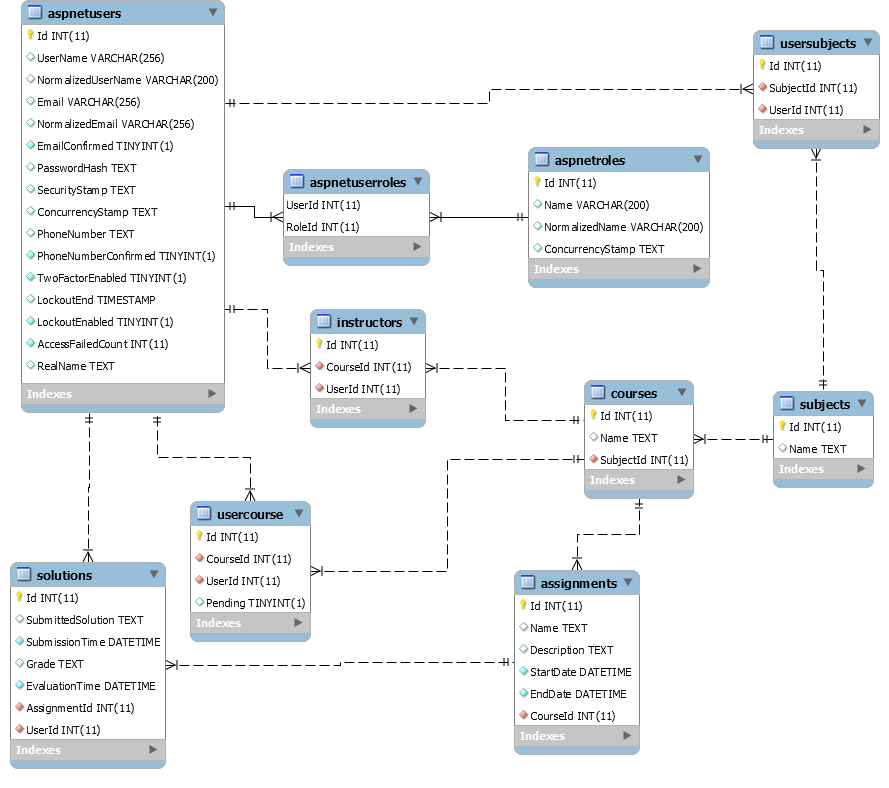
\includegraphics[width=1.0\textwidth]{developerguide/dbdiagram}
	\caption{Az adatbázis táblái}
	\label{fig:dbdiagram}
\end{figure}
\subsubsection{aspnetusers}
A \emph{Microsoft.AspNetCore.Identity.EntityFrameworkCore} programkönyvtár által automatikusan létrehozott tábla. A felhasználók adatait tárolja.
\begin{table}[H]
	\centering
	\begin{tabular}{ | m{0.25\textwidth} | m{0.25\textwidth} | m{0.40\textwidth} | }
		\hline
		\textbf{Mező neve} & \textbf{Típus} & \textbf{Leírás} \\
		\hline \hline
		Id & egész & Elsődleges kulcs \\
		\hline
		UserName & szöveg & Felhaszálónév (neptun kód) \\
		\hline
		Email & szöveg & Felhasználó e-mail címe \\
		\hline
		RealName & szöveg & Felhasználó neve \\
		\hline
		PasswordHash & szöveg & Felhasználó hashelt jelszava \\
		\hline
	\end{tabular}
	\caption{Adatbázis: felhasználók táblája}
	\label{tab:db-users}
\end{table}
\subsubsection{aspnetroles}
A \emph{Microsoft.AspNetCore.Identity.EntityFrameworkCore} programkönyvtár által automatikusan létrehozott tábla. A rendszerben használt szerepköröket tárolja.
\begin{table}[H]
	\centering
	\begin{tabular}{ | m{0.25\textwidth} | m{0.25\textwidth} | m{0.40\textwidth} | }
		\hline
		\textbf{Mező neve} & \textbf{Típus} & \textbf{Leírás} \\
		\hline \hline
		Id & egész & Elsődleges kulcs \\
		\hline
		Name & szöveg & Szerepkör megnevezése \\
		\hline
	\end{tabular}
	\caption{Adatbázis: szerepkörök táblája}
	\label{tab:db-roles}
\end{table}
\subsubsection{aspnetuserroles}
A \emph{Microsoft.AspNetCore.Identity.EntityFrameworkCore} programkönyvtár által automatikusan létrehozott tábla. Egy kapcsolótábla, mely tárolja a felhasználókhoz rendelt szerepköröket.
\begin{table}[H]
	\centering
	\begin{tabular}{ | m{0.25\textwidth} | m{0.25\textwidth} | m{0.40\textwidth} | }
		\hline
		\textbf{Mező neve} & \textbf{Típus} & \textbf{Leírás} \\
		\hline \hline
		UserId & egész & Elsődleges kulcs \\
		\hline
		RoleId & egész & Elsődleges kulcs \\
		\hline
	\end{tabular}
	\caption{Adatbázis: felhasználók és szerepkörök kapcsolótáblája}
	\label{tab:db-userroles-map}
\end{table}
\subsubsection{assignments}
Az \emph{assignments} tábla a csoportokhoz létrehozott beadandó feladatok adatainak tárolására szolgál.
\begin{table}[H]
	\centering
	\begin{tabular}{ | m{0.25\textwidth} | m{0.25\textwidth} | m{0.40\textwidth} | }
		\hline
		\textbf{Mező neve} & \textbf{Típus} & \textbf{Leírás} \\
		\hline \hline
		Id & egész & Elsődleges kulcs \\
		\hline
		Name & szöveg & A feladat neve \\
		\hline
		Description & szöveg & A feladat leírása \\
		\hline
		StartDate & dátum & A feladat elérésének dátuma \\
		\hline
		EndDate & dátum & A feladat határidejének dátuma \\
		\hline
		CourseId & egész & Arra vonatkozó kulcs, hogy a feladat melyik csoporthoz tartozik \\
		\hline
	\end{tabular}
	\caption{Adatbázis: feladatok táblája}
	\label{tab:db-assignments}
\end{table}
\subsubsection{courses}
A \emph{courses} tábla a tantárgyakhoz létrehozott csoportok adatait tárolja.
\begin{table}[H]
	\centering
	\begin{tabular}{ | m{0.25\textwidth} | m{0.25\textwidth} | m{0.40\textwidth} | }
		\hline
		\textbf{Mező neve} & \textbf{Típus} & \textbf{Leírás} \\
		\hline \hline
		Id & egész & Elsődleges kulcs \\
		\hline
		Name & szöveg & A csoport neve \\
		\hline
		SubjectId & egész & Arra vonatkozó kulcs, hogy a csoport melyik tantárgyhoz tartozik \\
		\hline
	\end{tabular}
	\caption{Adatbázis: csoportok táblája}
	\label{tab:db-courses}
\end{table}
\subsubsection{instructors}
A \emph{instructors} tábla egy kapcsolótábla, melyben a \emph{Gyakorlatvezető} szerepkörrel rendelkező felhasználókat kapcsoljuk a hozzájuk tartozó csoportokhoz. 
\begin{table}[H]
	\centering
	\begin{tabular}{ | m{0.25\textwidth} | m{0.25\textwidth} | m{0.40\textwidth} | }
		\hline
		\textbf{Mező neve} & \textbf{Típus} & \textbf{Leírás} \\
		\hline \hline
		Id & egész & Elsődleges kulcs \\
		\hline
		CourseId & egész & A csoportra vonatkozó kulcs \\
		\hline
		UserId & egész & A felhasználóra vonatkozó kulcs \\
		\hline
	\end{tabular}
	\caption{Adatbázis: gyakorlatvezetők táblája}
	\label{tab:db-instructors}
\end{table}
\subsubsection{solutions}
A \emph{solutions} tábla a feladatokra beadott megoldásokat tárolja.
\begin{table}[H]
	\centering
	\begin{tabular}{ | m{0.25\textwidth} | m{0.25\textwidth} | m{0.40\textwidth} | }
		\hline
		\textbf{Mező neve} & \textbf{Típus} & \textbf{Leírás} \\
		\hline \hline
		Id & egész & Elsődleges kulcs \\
		\hline
		SubmittedSolution & szöveg & A feladatra beadott megoldás \\
		\hline
		SubmissionTime & dátum & A megoldás beküldésének az időpontja \\
		\hline
		Grade & szöveg & A feladatra adott értékelése \\
		\hline
		EvaluationTime & dátum & A feladat értékelésének időpontja \\
		\hline
		AssignmentId & egész & Arra vonatkozó kulcs, hogy a megoldás melyik feladathoz tartozik\\
		\hline
		UserId & egész & Arra vonatkozó kulcs, hogy melyik felhasználó adta be a megoldást\\
		\hline
	\end{tabular}
	\caption{Adatbázis: megoldások táblája}
	\label{tab:db-solutions}
\end{table}
\subsubsection{subjects}
A \emph{subjects} tábla a rendszerben létrehozott tantárgyak adatait tárolja.
\begin{table}[H]
	\centering
	\begin{tabular}{ | m{0.25\textwidth} | m{0.25\textwidth} | m{0.40\textwidth} | }
		\hline
		\textbf{Mező neve} & \textbf{Típus} & \textbf{Leírás} \\
		\hline \hline
		Id & egész & Elsődleges kulcs \\
		\hline
		Name & szöveg & A tantárgy neve\\
		\hline
	\end{tabular}
	\caption{Adatbázis: megoldások táblája}
	\label{tab:db-subjects}
\end{table}
\subsubsection{usercourse}
A \emph{usercourse} tábla egy kapcsoló tábla, melyben a hallgatókat és a csoportok összerendelése valósul meg.
\begin{table}[H]
	\centering
	\begin{tabular}{ | m{0.25\textwidth} | m{0.25\textwidth} | m{0.40\textwidth} | }
		\hline
		\textbf{Mező neve} & \textbf{Típus} & \textbf{Leírás} \\
		\hline \hline
		Id & egész & Elsődleges kulcs \\
		\hline
		CourseId & egész & A csoportra vonatkozó kulcs\\
		\hline
		UserId & egész & A felhasználóra vonatkozó kulcs\\
		\hline
		Pending & igaz/hamis & Annak az értéke, hogy a felhasználónak a jelentkezése elfogadásra, vagy elutasításra került \\
		\hline
	\end{tabular}
	\caption{Adatbázis: hallgatók és csoportok kapcsolótáblája}
	\label{tab:db-usercourse}
\end{table}
\subsubsection{usersubjects}
A \emph{usersubjects} tábla egy kapcsoló tábla, melyben a tárgyfelelősök és a tantárgyak összerendelése valósul meg.
\begin{table}[H]
	\centering
	\begin{tabular}{ | m{0.25\textwidth} | m{0.25\textwidth} | m{0.40\textwidth} | }
		\hline
		\textbf{Mező neve} & \textbf{Típus} & \textbf{Leírás} \\
		\hline \hline
		Id & egész & Elsődleges kulcs \\
		\hline
		SubjectId & egész & A tantárgyra vonatkozó kulcs\\
		\hline
		UserId & egész & A felhasználóra vonatkozó kulcs\\
		\hline
	\end{tabular}
	\caption{Adatbázis: tárgyfelelősök és tantárgyak kapcsolótáblája}
	\label{tab:db-usersubjects}
\end{table}
\section{Model réteg}
\label{sec:model}
\subsection{Üzleti logika}
Az üzleti logikát megvalósító objektumokat az \emph{ASS.BLL.Interfaces} és az \emph{ASS.BLL.Services} névtérben tároljuk. Az üzleti logikát szerepkörökre bontva valósítjuk meg. Minden szerepkörhöz tartozik egy \emph{interface}, mely leírja a szerepkörhöz tartozó funkciók metódusait, valamint egy osztály, ami implementálja az adott \emph{interface}-t. Az \emph{interface}-ket megvalósító osztályok a \emph{BaseService} osztályból származnak le\footnote{Kivéve a \emph{LoginService} osztályt.} (\ref{fig:bll-baseservice} ábra), melyben azok a funkcionalitások kerültek implementálásra, amiket minden egyes szerepkörhöz tartozó \emph{service} osztálynak meg kell valósítania. Ezeket a \emph{service} osztályokat az alkalmazás \emph{IoC} (\emph{Inversion of Control}) konténerébe \cite{IoC} regisztráljuk. Ezáltal a vezérlő osztályok rendelkeznek a hozzájuk tartozó \emph{service} osztály egy példányával, melyet konstruktoron keresztüli függőségi befecskendezéssel kapnak meg. A vezérlő osztályok ezen \emph{service} osztályok metódusainak segítségével dolgozzák fel a kliens kéréseit és állítják elő a megfelelő válaszokat.
\begin{figure}[H]
	\centering
	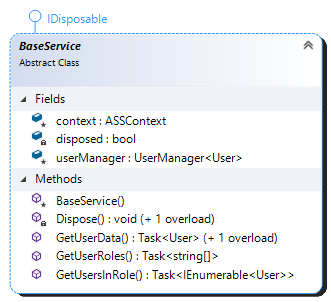
\includegraphics[width=0.7\textwidth]{developerguide/baseservice}
	\caption{Service osztályok őse}
	\label{fig:bll-baseservice}
\end{figure}
\subsubsection{BaseService osztály}
\begin{description}
	\item[GetUserData(ClaimsPrincipal):] paraméterül a bejelentkezett felhasználót\footnote{\href{https://docs.microsoft.com/en-us/dotnet/api/system.security.claims.claimsprincipal?view=netcore-3.1}{Ezen a linken} elolvashatjuk a \emph{ClaimsPrincipal} osztály dokumentációját.} kapja a metódus, majd eredményül a paraméterül kapott felhasználónak az adataival tér vissza.
	\item[GetUserData(int):] az előbbi metódus túlterhelése, itt a keresendő felhasználó egyedi kulcsát kapja a metódus paraméterül.
	\item[GetUserRoles(ClaimsPrincipal):] paraméterül a bejelentkezett felhasználót kapja, majd a felhasználó szerepköreivel tér vissza.
	\item[GetUsersInRole(Role):] paraméterül egy \emph{Role enum} értéket kap, majd a paraméterül kapott szerepkörrel rendelkező felhasználókkal tér vissza.
	\item[Dispose():] az \emph{IDisposeable interface} metódusa, mely gondoskodik a külső erőforrások felszabadításáról.
\end{description}
\subsubsection{LoginService osztály}
Ez az osztály felelős az alkalmazásba való bejelentkeztetésért, kijelentkeztetésért, valamint a bejelentkeztetett felhasználó fontos adatainak (felhasználónév, név, szerepkörök) lekérdezéséért, hogy a felhasználó munkamenetében (angolul \emph{session}) tudja tárolni a rendszer.
\begin{description}
	\item[CreateFullUserName(ClaimsPrincipal):] paraméterül a bejelentkezett felhasználót kapja, majd a felhasználó polgári nevéből és felhasználónevéből képzett \emph{string}-el tér vissza.
	\item[CreateUserRolesJson(ClaimsPrincipal):] paraméterül a bejelentkezett felhasználót kapja, majd a felhasználó szerepköreivel tér vissza.
	\item[SignIn(string,string,bool,bool):] paraméterül a bejelentkezési adatokat kapja, majd egy igaz/hamis értékkel tér vissza, ami a bejelentkezés sikerességét jelzi.
	\item[SignOut():] kijelentkezteti a felhasználót az alkalmazásból.
\end{description}
\begin{figure}[H]
	\centering
	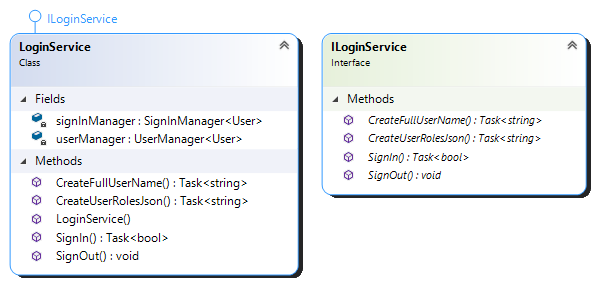
\includegraphics[width=1.0\textwidth]{developerguide/loginservice}
	\caption{LoginService osztály és interface}
	\label{fig:bll-loginservice}
\end{figure}
\subsubsection{AdminService osztály}
\begin{description}
	\item[CreateSubject(string{[]},string):] paraméterül \emph{tárgyfelelős}i szerepkörrel rendelkező felhasználók felhasználóneveit és a létrehozandó tantárgy nevét kapja. A metódus leellenőrzi, hogy a paraméterül kapott tantárgy név létezik-e már a rendszerben, ha nem, akkor a rendszer létrehozza a tantárgyat, egyébként kivétel váltódik ki.
	\item[GetSubjects():] a metódus visszatérési értéke a rendszerben létrehozott összes tantárgy.
	\item[UpdateSubject(int,string,string{[]}):] paraméterül egy tantárgy egyedi azonosítóját, tantárgy nevet és \emph{tárgyfelelős}i szerepkörrel rendelkező felhasználók felhasználóneveit kapja. A metódus módosítja a kapott paraméterek alapján a tantárgy adatait, ha az új tantárgynév még nem foglalt, egyébként kivétel váltódik ki.
	\item[DeleteSubject(int):] paraméterül egy tantárgy egyedi azonosítóját kapja, majd a megfelelő tantárgyat a metódus törli a rendszerből.
	\item[GetAllUser():] a metódus listázza a rendszerben tárolt összes felhasználót.
	\item[GetUserRoles(int):] paraméterül egy felhasználó egyedi azonosítóját kapja, majd a megfelelő felhasználó szerepköreivel tér vissza.
	\item[CreateUser(string,string,string,string,string{[]}):] a metódus egy új felhasználót hoz létre a rendszerben a paraméterül kapott adatok alapján.
	\item[UpdateUser(int,string,string,string,string{[]}):] paraméterül egy felhasználó adatait kapja (egyedi azonosító, felhasználónév, polgári név, e-mail cím, szerepkörök). A metódus a megfelelő felhasználó adatait módosítja.
\end{description}
\begin{figure}[H]
	\centering
	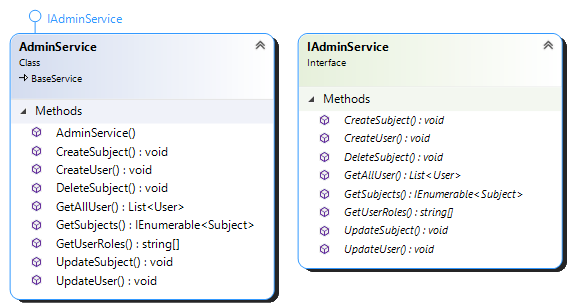
\includegraphics[width=1.0\textwidth]{developerguide/adminservice}
	\caption{AdminService osztály és interface}
	\label{fig:bll-adminservice}
\end{figure}
\subsubsection{TeacherService osztály}
Ez az osztály implementálja a \emph{tárgyfelelős}i szerepkörhöz tartozó funkciókat.
\begin{description}
	\item[CreateCourse(string{[]},int,string):] paraméterül felhasználónevek tömbjét, egy tantárgynak az egyedi azonosítóját illetve egy csoportnevet kap. A metódus létrehozza a paraméterül kapott tantárgyhoz az új csoportot, amennyiben ez lehetséges. Ha sikeres volt a csoport létrehozása, akkor a paraméterül kapott felhasználókat hozzárendeli a csoporthoz.
	\item[GetSubjects(ClaimsPrincipal):] paraméterül kap egy bejelentkezett felhasználót, majd a hozzárendelt tantárgyakkal tér vissza egy listában.
	\item[GetCourse(int):] paraméterül egy csoportnak az egyedi azonosítóját kapja, majd visszatér ezen csoport adataival.
	\item[EditCourse(int,string,string{[]}):] paraméterül egy csoportnak az egyedi azonosítóját, a csoport nevét, és gyakorlatvezetők felhasználóneveit kapja. A metódus a paraméterül kapott adatokkal módosítja a megfelelő csoportot. 
\end{description}
\begin{figure}[H]
	\centering
	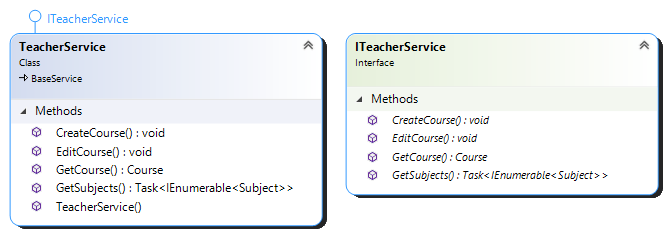
\includegraphics[width=1.0\textwidth]{developerguide/teacherservice}
	\caption{TeacherService osztály és interface}
	\label{fig:bll-teacherservice}
\end{figure}
\subsubsection{InstructorService osztály}
\begin{description}
	\item[GetPendingList(ClaimsPrincipal):] paraméterül a bejelentkezett felhasználót kapja, visszatérési értéke a felhasználóhoz tartozó csoportba jelenkezett hallgatók listája.
	\item[ProcessPendingStatus(int,bool):] paraméterül a jelentkezéseket tároló kapcsolótábla (\emph{UserCourses}) egyedi azonosítóját és egy igaz/hamis érték kap. A metódus az igaz/hamis érték alapján frissíti a megfelelő jelentkezési státuszt. Az igaz érték a jelentkezés elfogadását jelenti, a hamis pedig az elutasítást.
	\item[GetCourses(ClaimsPrincipal):] paraméterül a bejelentkezett felhasználót kapja, eredményül pedig a felhasználóhoz tartozó csoportokkal tér vissza.
	\item[CreateAssignment(string,string,DateTime,DateTime,int{[]}):] paraméterül egy feladatnak az adatait kapja. A metódus leellenőrzi, hogy a feladat elérésének a dátuma korábban van-e mint a beadási határidő, ha igen akkor elmenti a feladatot, ha nem teljesül a feltétel, akkor kivétel váltódik ki.
	\item[GetAssignment(int,int,ClaimsPrincipal):] paraméterül egy csoport és egy feladat egyedi azonosítóját valamint a bejelentkezett felhasználót kapja. A metódus a paraméterül kapott feladat adataival tér vissza, amennyiben a felhasználó gyakorlatvezetője a paraméterül kapott csoportnak, egyébként kivétel váltódik ki.
	\item[GetStudent(int):] paraméterül egy hallgató egyedi azonosítóját kapja, visszatérési értéke a megfelelő felhasználó adatai.
	\item[EvaluateAssignment(int,string,DateTime,ClaimsPrincipal):] paraméterül egy feladat egyedi azonosítóját, a feladatra beadott megoldás értékelését, az értékelésnek az időpontját és a bejelentkezett felhasználót kapja. A metódus ellenőrzi, hogy az a felhasználó, aki az értékelést végrehajtja, a kiiírt feladat csoportjának a gyakorlatvezetője-e. Ha igen, elmentődik az értékelés, egyébként kivétel váltódik ki.
\end{description}
\begin{figure}[H]
	\centering
	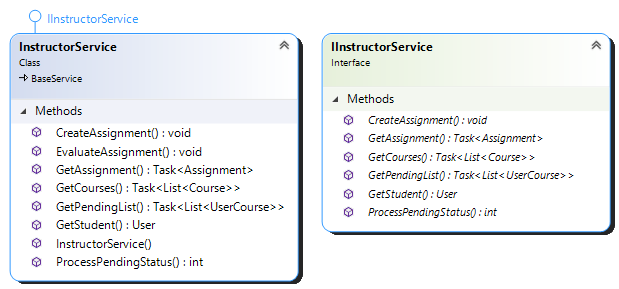
\includegraphics[width=1.0\textwidth]{developerguide/instructorservice}
	\caption{InstructorService osztály és interface}
	\label{fig:bll-instructorservice}
\end{figure}
\subsubsection{StudentService osztály}
Ez az osztály implementálja a \emph{hallgató}i szerepkörnek a funkcióit.
\begin{description}
	\item[GetCourses(ClaimsPrincipal):] paraméterül a bejelentkezett felhasználót kapja meg, majd a felhasználóhoz tartozó csoportokkal tér vissza.
	\item[CourseRegistration(int{[]},ClaimsPrincipal):] paraméterül csoportok egyedi azonosítójának a tömbjét és a bejelentkezett felhasználót kapja, majd a felhasználót felveszi a paraméterül kapott csoportokba\footnote{Ezen a ponton még a hallgató csak jelentkezést adott le az adott csoport(ok)ba.}.
	\item[Read\_AssignmentGrid(ClaimsPrincipal):] paraméterül a bejelentkezett felhasználót kapja, majd a hozzá tartozó csoportok listájával tér vissza.
	\item[GetAssignment(int,ClaimsPrincipal):] paraméterül egy feladatnak az egyedi azonosítóját és a bejelentkezett felhasználót kapja, majd visszatér a paraméterül kapott feladat adataival, ha a felhasználó tagja annak a csoportnak, amelyiket lekérdeztük.
	\item[SubmitSolution(int,ClaimsPrincipal,string,DateTime):] paraméterül egy feladat egyedi azonosítóját, a bejelentkezett felhasználót, a feladat megoldását és a beadás időpontját kapja. A metódus leellenőrzi, hogy a beadás időpontja korábbi-e mint a feladat beadási határideje. Amennyiben helyes a beadási idő, elmenti a beadott megoldást, ellenkező esetben kivétel váltódik ki.
\end{description}
\begin{figure}[H]
	\centering
	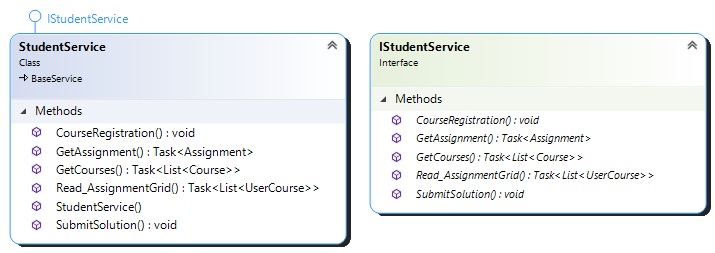
\includegraphics[width=1.0\textwidth]{developerguide/studentservice}
	\caption{StudentService osztály és interface}
	\label{fig:bll-studentservice}
\end{figure}
\subsection{Adatok megjelenítésére szolgáló modellek}
Az adatok megjelenítésére adatátviteli objektumok\footnote{\url{https://en.wikipedia.org/wiki/Data_transfer_object}} (angolul \emph{Data transfer object \(DTO\)}) kerülnek definiálásra. Feladatuk a folyamatok között közvetíteni a szükséges adatokat. Jelen esetben a vezérlő meghívja az üzleti logika megfelelő metódusát a kérés során, majd egy ilyen \emph{DTO} osztályba csomagolja az üzleti logika által visszaadott \emph{entitás}\footnote{Azokat az osztályokat nevezzük \emph{entitás} osztálynak, melyekből az adatbázis táblák képződnek le.} osztályokban tárolt adatokat és ezt az objektumot kapja meg a nézet, hogy megtudja jeleníteni a kliens számára az adatokat. Ezeket az osztályokat a \emph{ASS.WEB.Models.DTOs} névtérben tároljuk.
\subsection{Adatok bevitelére szolgáló modellek}
Az adatok bevitele nézetmodellek (angolul \emph{viewmodel}) segítségével valósul meg. A nézetmodelleket a \emph{ASS.WEB.Models.ViewModels} névtérben tároljuk. A nézetmodellek tulajdonságaira (angolul \emph{property}) megszabhatunk (egy vagy több) attribútomot, melyet a \emph{System.ComponentModel.DataAnnotations} névtérből érünk el. Az attribútomok használatával egyszerűen tudjuk validálni nézetmodelljeinket, vagy a valadiációs hibaüzenetek testreszabni. Ezt a \emph{.NET} keretrendszer biztosítja. Ugyanis fontos a felhasználó által kitöltött űrlapok ellenőrzése, hogy hibás adatok ne kerülhessenek a rendszerbe. A nézetmodelleket a rendszer az űrlapoknál használja fel, tehát a nézetmodellek egy-egy kitöltött űrlap adatait képes tárolni. Az attribútomok leírását a Microsoft hivatalos honlápján részletesen el lehet olvasni \cite{DataAnnotations}.
\lstset{caption={Példa az attribútomok használatára}, label=src:loginviewmodel}
\begin{lstlisting}[language={[Sharp]C}]
using System.ComponentModel.DataAnnotations;

namespace ASS.WEB.Models.ViewModels
{
	public class LoginViewModel
	{
		[Required(ErrorMessageResourceType = typeof(Resources.Models.ViewModels.LoginViewModel),ErrorMessageResourceName = "UsernameRequired")]
		[StringLength(maximumLength: 10, MinimumLength = 5, ErrorMessageResourceType = typeof(Resources.Models.ViewModels.LoginViewModel), ErrorMessageResourceName = "UsernameLengthMessage")]
		[Display(ResourceType = typeof(Resources.Models.ViewModels.LoginViewModel), Name = "Username")]
		public string Username { get; set; }

		...
	}
}
\end{lstlisting}
\subsection{Egyéb segédosztályok}
Az alkalmazásban definiálásra kerülnek egyéb segédosztályok és egy felsorolási típus (angolul \emph{enum}), melyeket az alább ábrán látható helyen találunk.
\begin{center}
	\begin{forest}
		for tree={
			font=\ttfamily,
			grow'=0,
			child anchor=west,
			parent anchor=south,
			anchor=west,
			calign=first,
			edge path={
			\noexpand\path [draw, \forestoption{edge}]
			(!u.south west) +(7.5pt,0) |- node[fill,inner sep=1.25pt] {} (.child anchor)\forestoption{edge label};
			},
			before typesetting nodes={
			if n=1
				{insert before={[,phantom]}}
				{}
			},
			fit=band,
			before computing xy={l=15pt},
		}
		[ASS
			[ASS.Common/
				[Enums/
					[Role.cs]
				]
				[Helpers/
					[CultureCodeMapping.cs]
				]
				[Settings/
					[IdentitySettings.cs]
					[LockoutSettings.cs]
					[PasswordSettings.cs]
					[UserSettings.cs]
				]
			]
		]
	\end{forest}
\end{center}
\subsubsection{Role.cs}
A \emph{Role} felsorolási típus segítségével definiáljuk a rendszerben tárolt szerepköröket. Ugyanis így a forráskódban nem szükséges beégetett szövegeket használnunk a szerepkörökre\footnote{Ez alól kivétel az \emph{Authorize} attribútom, mivel az attribútomokban a keretrendszer csak konstans értékeket enged használni.}.
\lstset{caption={Szerepkörök felsorolási típusa}, label=src:roleenum}
\begin{lstlisting}[language={[Sharp]C}]
namespace ASS.Common.Enums
{
	public enum Role
	{
		Admin,
		Teacher,
		Instructor,
		Student
	}
}
\end{lstlisting}
Továbbá a \emph{Role enum} segítségével egy ciklussal könnyedén tudjuk az adatbázisba perzisztálni az \emph{enum} értékeit.
\lstset{caption={Szerepkörök tárolása az adatbázisba (DbInitializer.cs)}, label=src:roles}
\begin{lstlisting}[language={[Sharp]C}]
...
foreach (Role item in Enum.GetValues(typeof(Role)))
{
	context.Roles.Add(new IdentityRole<int>() { Name = item.ToString(), NormalizedName = item.ToString() });
}
...
\end{lstlisting}
\subsubsection{CultureCodeMapping.cs}
A \emph{CultureCodeMapping} egy statikus segédosztály, amely egy nyelvi kódból a nyelvet adja vissza. Ezt a segédosztályt a lokalizációnál használjuk, hogy a felületen ne a nyelvi kód (pl.: \emph{hu-HU}) jelenjen meg, hanem az adott nyelv neve.
\lstset{caption={CultureCodeMapping osztály}, label=src:culturecodemapping}
\begin{lstlisting}[language={[Sharp]C}]
namespace ASS.Common.Helpers
{
	public static class CultureCodeMapping
	{
		public static string CultureCodeToCountryName(string cultureCode)
		{
			switch (cultureCode)
			{
				case "hu-HU":
					return "Magyar";
				case "en-US":
					return "English";
				default:
					return "Ismeretlen";
			}
		}
	}
}
\end{lstlisting}
\subsubsection{Settings osztályok}
A \emph{Microsoft.AspNetCore.Identity} \cite{IdentityOptions} lehetővé tesz különböző konfigurációk beállítását a felhasználói fiókokra. Például jelszóra vonatkozó konfigurációkat (minimum hossz, kötelező számot tartalmaznia stb), felhasználóra vonatkozó megszorításokat (minden felhasználó egyedi e-mail címmel rendelkezzen) és hibás bejelentkezés esetén konfigurálhatjuk a felhasználó kizárását az alkalmazásből (a kizárás időtartama). Ezen konfigurációk könnyű állíthatósága érdekében a konfigurációs értékek az alkalmazás konfigurációs fájljába (\emph{appsettings.json}) kiszervezésre kerültek.
\lstset{caption={Felhasználói fiók konfigurációs beállításai}, label=src:identityoptions}
\begin{lstlisting}[language=json]
...
"User": {
	"RequireUniqueEmail": false
},
"Password": {
	"RequiredLength": 1,
	"RequireLowercase": false,
	"RequireUppercase": false,
	"RequireDigit": false,
	"RequireNonAlphanumeric": false,
	"RequiredUniqueChars" : 1
},
"Lockout": {
	"AllowedForNewUsers": false,
	"DefaultLockoutTimeSpanInMins": 30,
	"MaxFailedAccessAttempts": 10
}
...
\end{lstlisting}
Ugyanis így a kód módosítása nélkül tudjuk változtatni ezen konfigurációs beállításokat és nem kell a változások után újra fordítani az alkalmazást, hanem elengedő csak újraindítani, hiszen a forráskód nem változott. Ezeket a beállításokat az alkalmazás indításakor kerül kiolvasásra az \emph{appsettings.json} fájlból, majd szerializálja a megfelelő objektumba (\emph{IdentitySettings} osztály) az adatokat. Továbbá egyszerre több fajta konfigurációs beállítást megadhatunk, annak függvényében, hogy az alkalmazás milyen módban fut\footnote{Ezt a beállítást is az \emph{appsettings.json} fájlban állíthatjuk} (\ref{src:appmode} forráskód).
\lstset{caption={Alkalmazás futási módja}, label=src:appmode}
\begin{lstlisting}[language=json]
"Mode": "Development",
...
\end{lstlisting}
Ennek használatával elég csak a módot változtatni, nem kell az összes \emph{IdentitySettings}-hez tartozó értéket módosítani.
\section{Vezérlő réteg}
\label{sec:controller}
\subsection{\emph{Home} vezérlő}
A \emph{Home} vezérlő (\ref{fig:homecontroller} ábra) az alkalmazás alap funkcionalitásait implementálja, mint például a bejelentkezés vagy a kijelentkezés. Ez a vezérlő mindenki számára elérhető, nincs szerepkörhöz kötve.
\begin{description}
	\item[{[HttpGet]} Index():] visszatér az alkalmazás főoldalával.
	\item[{[HttpPost]} Login(LoginViewModel):] paraméterül a bejelentkezési adatokat kapja (felhasználónév, jelszó), majd a kapott adatokkal megpróbálja bejelentkeztetni az alkalmazásba a felhasználót, sikeres bejelentkezés esetén a szerepkörének megfelelő kezdőoldalra irányítja, egyébként jelzi a hibát a felhasználónak.
	\item[{[HttpPost]} CultureManagment(string):] paraméterül egy nyelvi kódot kap (pl.: hu-HU), majd \emph{sütibe} menti a kapott nyelvi kódot, és visszatér az alkalmazás főoldalával. 
	\item[{[HttpGet]} Error(string):] paraméterül a keletkezett hibának az azonosítóját kapja, majd visszatér az alkalmazás hibaoldalával.
	\item[{[HttpGet]} AccessDenied():] az alkalmazás \emph{jogosulatlan kérés} oldalával tér vissza.
	\item[{[HttpGet]} Logout():] kijelentkezteti a felhasználót, majd visszatér az alkalmazás főoldalával.
\end{description}
\begin{figure}[H]
	\centering
	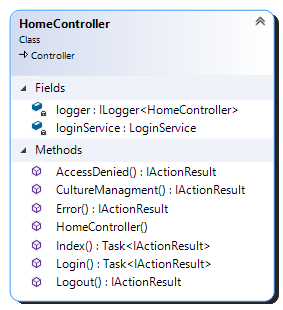
\includegraphics[width=0.6\textwidth]{developerguide/homecontroller}
	\caption{\emph{Home} vezérlő}
	\label{fig:homecontroller}
\end{figure}
\subsection{\emph{Base} vezérlő}
A vezérlők őse\footnote{Leszámítva a \emph{Home} vezérlőt.} (\ref{fig:basecontroller} ábra), mely azokat a funkcionalitásokat valósítja meg, amellyel minden szerepkörhöz tartozó vezérlőnek tudnia kell.
\begin{description}
	\item[{[HttpGet]} Profile():] lekéri a bejelentkezett felhasználó adatait, majd visszatér személyes adatokat megjelenítő oldallal.
	\item[{[HttpPost]} CultureManagment(string):] paraméterül egy nyelvi kódot kap (pl.: hu-HU), majd \emph{sütibe} menti a kapott nyelvi kódot, és visszatér a személyes adatokat megjelenítő oldallal. 
\end{description}
\begin{figure}[H]
	\centering
	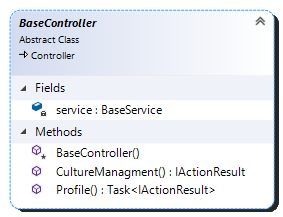
\includegraphics[width=0.6\textwidth]{developerguide/basecontroller}
	\caption{\emph{Base} vezérlő}
	\label{fig:basecontroller}
\end{figure}
\subsection{\emph{Admin} vezérlő}
Az \emph{Admin} vezérlőt csak rendszergazdai szerepkörrel rendelkező felhasználók érhetik el.
\begin{description}
	\item[{[HttpGet]} Index():] a rendszergazdai szerepkör főoldalával tér vissza.
	\item[{[HttpGet]} GetTeachers():] lekéri a rendszerben szereplő tárgyfelelősi szerepkörrel rendelkező felhasználókat és ennek eredményével tér vissza.
	\item[{[HttpGet]} CreateSubject():] a tantárgyak létrehozására alkalmas felületet adja vissza.
	\item[{[HttpPost]} CreateSubject(CreateSubjectViewModel):] a tantárgy létrehozásának fogadása, ellenőrzi az adatok helyességét. Sikeres adatrögzítés után átirányítás történik a szerepkör főoldalára, egyébként jelzi a hibát a felhasználónak.
	\item[{[HttpGet]} GetSubjects():] lekéri a rendszerben szereplő tantárgyakat és ennek eredményével tér vissza.
	\item[{[HttpPost]} DeleteSubject(string):] paraméterül egy \emph{Json string}-et\footnote{\href{https://www.json.org/json-en.html}{Javascript Object Notation}} kap melyben a törölni kívánt tantárgy adatai vannak tárolva. Ezt a tárgyat törli a rendszerből.
	\item[{[HttpPost]} UpdateSubject(string):] paraméterül egy \emph{Json string}-et kap melyben a módosítani kívánt tantárgy adatai vannak, sikertelen módosítás esetén átirányítás történik a hibaoldalra.
	\item[{[HttpGet]} Read\_UserGrid():] lekéri a rendszerben tárolt felhasználókat és ennek eredményével tér vissza.
	\item[{[HttpGet]} CreateUser():] a felhasználók létrehozására alkalmas felületet adja vissza.
	\item[{[HttpPost]} CreateUser(CreateUserViewModel):] a felhasználó létrehozásának fogadása, ellenőrzi az adatok helyességét. Sikeres rögzítés esetén átirányítás történik a szerepkör főoldalára, egyébként jelzi a hibát a felhasználónak.
	\item[{[HttpGet]} GetAllRole():] lekéri a rendszerben található szerepköröket és ennek eredményével tér vissza.
	\item[{[HttpGet]} UpdateUser(int):] paraméterül egy felhasználó egyedi azonosítóját kapja, majd lekéri a paraméterül kapott felhasználó adatait. Ezután a felhasználó módosítására alkalmas felületet adja vissza, a szükséges adatokkal (a felhasználó adatai).
	\item[{[HttpPost]} UpdateUser(UpdateUserViewModel):] a felhasználó módosításának fogadása, ellenőrzi az adatok helyességét. Sikeres rögzítés esetén átirányítás történik a szerepkör főoldalára, egyébként jelzi a hibát a felhasználónak.
\end{description}
\begin{figure}[H]
	\centering
	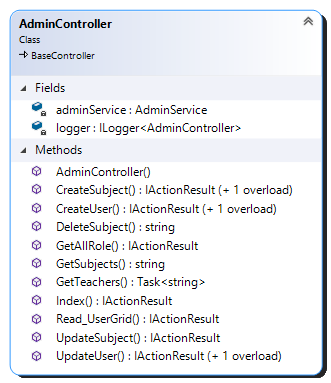
\includegraphics[width=0.6\textwidth]{developerguide/admincontroller}
	\caption{\emph{Admin} vezérlő}
	\label{fig:admincontroller}
\end{figure}
\subsection{\emph{Instructor} vezérlő}
Az \emph{Instructor} vezérlőt csak gyakorlatvezetői szerepkörrel rendelkező felhasználók érhetik el.
\begin{description}
	\item[{[HttpGet]} Index():] a gyakorlatvezetői szerepkör főoldalával tér vissza.
	\item[{[HttpGet]} CreateAssignment():] feladat létrehozására alkalmas felületet adja vissza.
	\item[{[HttpPost]} CreateAssignment(CreateAssignmentViewModel):] a feladat létrehozásának fogadása és ellenőrzi az adatok helyességét. Sikeres rögzítés esetén átirányítás történik a szerepkör főoldalára, egyébként jelzi a hibát a felhasználónak.
	\item[{[HttpGet]} GetCourses():] lekéri a bejelentkezett felhasználóhoz tartozó csoportokat és ennek eredményével tér vissza.
	\item[{[HttpGet]} GetPendingList():] lekéri a bejelentkezett felhasználóhoz tartozó csoportokra jelentkezett felhasználókat és ennek eredményével tér vissza.
	\item[{[HttpGet]} EvaluateAssignment(int, int, int):] a paraméterül kapott egyedi azonosítók alapján (csoport,feladat,hallgató) lekéri a megfelelő adatokat és a feladat értékelésére alkalmas felületet adja vissza ezen adatokkal.
	\item[{[HttpPost]} EvaluateAssignment(int, string):] a feladat értékelésének fogadása, ellenőrzi az adatok helyességét. Sikeres rögzítés esetén átirányítás történik a szerepkör főoldalára, egyébként jelzi a hibát a felhasználónak.
	\item[{[HttpPost]} ProcessPendingStatus(int, bool):] a csoportba való jelentkezés bírálatának fogadása.
\end{description}
\begin{figure}[H]
	\centering
	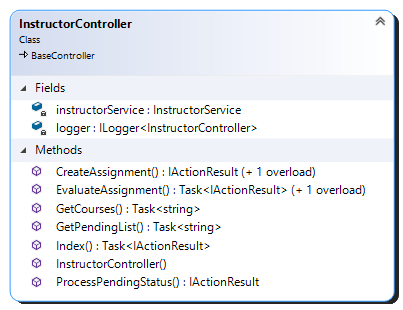
\includegraphics[width=0.6\textwidth]{developerguide/instructorcontroller}
	\caption{\emph{Instructor} vezérlő}
	\label{fig:instructorcontroller}
\end{figure}
\subsection{\emph{Teacher} vezérlő}
A \emph{Teacher} vezérlőt csak tárgyfelelősi szerepkörrel rendelkező felhasználók érhetik el.
\begin{description}
	\item[{[HttpGet]} Index():] a tárgyfelelősi szerepkör főoldalával tér vissza.
	\item[{[HttpGet]} CreateCourse():] csoport létrehozására alkalmas felületet adja vissza.
	\item[{[HttpPost]} CreateCourse(CreateCourseViewModel):] csoport létrehozásának fogadása, ellenőrzi az adatok helyességét. Sikeres rögzítés esetén átirányítás történik a szerepkör főoldalára, egyébként jelzi a hibát a felhasználónak.
	\item[{[HttpGet]} Read\_SubjectGrid():] a bejelentkezett felhasználóhoz tartozó tantárgyakat és a hozzátartozó adatokat kéri le és ennek eredményével tér vissza.
	\item[{[HttpGet]} GetSubjects():] a bejelentkezett felhasználóhoz tartozó tantárgyak neveit és egyedi azonosítóit kéri le és ennek eredményével tér vissza.
	\item[{[HttpGet]} GetInstructors():] a rendszerben tárolt gyakorlatvezetői szerepkörrel rendelkező felhasználókat kéri le és ennek eredményével tér vissza.
	\item[{[HttpGet]} EditCourse(int):] paraméterül egy csoport egyedi azonosítóját kapja, majd a megfelelő csoport adatait kéri le és a csoport módosítására alkalmas felületet adja vissza ezen adatokkal.
	\item[{[HttpPost]} EditCourse(EditCourseViewModel):] a csoport módosításának fogadása, ellenőrzi az adatok helyességét. Sikeres rögzítés esetén átirányítás történik a szerepkör főoldalára, egyébként jelzi a hibát a felhasználónak.
\end{description}
\begin{figure}[H]
	\centering
	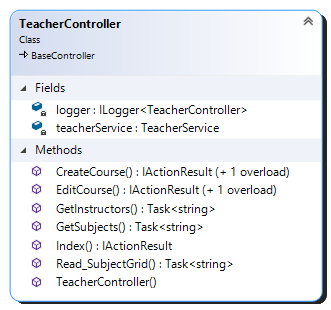
\includegraphics[width=0.6\textwidth]{developerguide/teachercontroller}
	\caption{\emph{Teacher} vezérlő}
	\label{fig:teachercontroller}
\end{figure}
\subsection{\emph{Student} vezérlő}
A \emph{Student} vezérlőt csak hallgatói szerepkörrel rendelkező felhasználók érhetik el.
\begin{description}
	\item[{[HttpGet]} Index():] a hallgatói szerepkör főoldalával tér vissza.
	\item[{[HttpGet]} GetCourses():] lekérdezi a bejelentkezett felhasználóhoz tartozó csoportokat és ennek eredményével tér vissza.
	\item[{[HttpGet]} CourseRegistration():] a csoportba való jelentkezésre alkalmas felületet adja vissza.
	\item[{[HttpPost]} CourseRegistration(CourseRegistrationViewModel):] a csoportba való jelentkezés fogadása, ellenőrzi az adatok helyességét. Sikeres rögzítés esetén átirányítás történik a szerepkör főoldalára, egyébként jelzi a hibát a felhasználónak.
	\item[{[HttpGet]} Read\_AssignmentGrid():] lekérdezi a bejelentkezett felhasználóhoz tartozó csoportokat és annak adatait, majd ennek eredményével tér vissza.
	\item[{[HttpGet]} Assignment(int):] paraméterül egy feladat egyedi azonosítóját kapja, majd lekéri a feladat adatait, és ezeket az adatokat, valamint a feladat megjelenítésére és a megoldás beküldésére alkalmas felületet adja vissza.
	\item[{[HttpPost]} SubmitSolution(SolutionSubmissionViewModel):] a feladatra való megoldásának fogadása, ellenőrzi az adatok helyességét. Sikeres rögzítés esetén átirányítás történik a szerepkör főoldalára, egyébként jelzi a hibát a felhasználónak.
\end{description}
\begin{figure}[H]
	\centering
	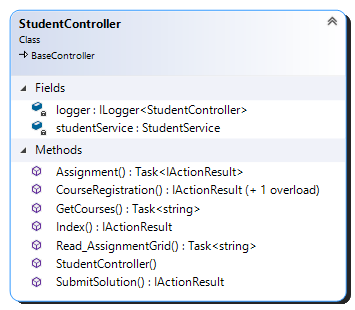
\includegraphics[width=0.6\textwidth]{developerguide/studentcontroller}
	\caption{\emph{Student} vezérlő}
	\label{fig:studentcontroller}
\end{figure}
\section{Nézet réteg}
\label{sec:view}
Ez a réteg felelős az adatok megjelenítéséért, illetve az egész alkalmazás kinézetéért. A nézeteket a \emph{Views} mappában találjuk vezérlők szerinti almappákba csoportosítva, valamint a megosztott nézeteket a \emph{Shared} mappában. A nézetek megvalósításakor \emph{Razor} \cite{Razor} szintaxist is használnunk, mellyel \emph{C\#} forráskódot illeszthetünk a \emph{HTML} alapú nézetekbe, ezzel megvalósítva a nézetek dinamikus működését.
\begin{center}
	\begin{forest}
		for tree={
			font=\ttfamily,
			grow'=0,
			child anchor=west,
			parent anchor=south,
			anchor=west,
			calign=first,
			edge path={
			\noexpand\path [draw, \forestoption{edge}]
			(!u.south west) +(7.5pt,0) |- node[fill,inner sep=1.25pt] {} (.child anchor)\forestoption{edge label};
			},
			before typesetting nodes={
			if n=1
				{insert before={[,phantom]}}
				{}
			},
			fit=band,
			before computing xy={l=15pt},
		}
		[Views/
			[Admin/]
			[Home/]
			[Instructor/]
			[Shared/]
			[Student/]
			[Teacher/]
		]
	\end{forest}
\end{center}
\subsection{\emph{Home} vezérlő nézetei}
\begin{description}
	\item[Index:] az alkalmazás főoldala, továbbá ezen a nézeten lehet bejelentkezni és az alkalmazás nyelvét módosítani.
\end{description}
\subsection{\emph{Admin} vezérlő nézetei}
\begin{description}
	\item[Index:] A rendszergazdai szerepkör főoldalának nézete.
	\item[CreateSubject:] tantárgyak létrehozására szolgáló nézet, amely egy űrlapot tartalmaz, ami a megfelelő vezérlőnek továbbítja a bevitt adatokat.
	\item[CreateUser:] felhasználók létrehozására szolgáló nézet, amely egy űrlapot tartalmaz, ami a megfelelő vezérlőnek továbbítja a bevitt adatokat.
	\item[UpdateUser:] felhasználók adatainak módosítására szolgáló nézet, amely egy űrlapba tölti a felhasználó aktuális adatait, majd a megfelelő vezérlőnek továbbítja az adatokat.
\end{description}
\subsection{\emph{Instructor} vezérlő nézetei}
\begin{description}
	\item[Index:] a gyakorlatvezetői szerepkör főoldalának nézete.
	\item[CreateAssignment:] feladat létrehozására szolgáló nézet, amely egy űrlapot tartalmaz, ami a megfelelő vezérlőnek továbbítja a bevitt adatokat. 
	\item[EvaluateAssignment:] feladat értékelésére szolgáló nézet, mely megjeleníti a hallgató beadott munkáit, valamint tartalmaz egy űrlapot, amivel az értékelést tudjuk elküldeni a megfelelő vezérlőnek.
\end{description}
\subsection{\emph{Teacher} vezérlő nézetei}
\begin{description}
	\item[Index:] a tárgyfelelősi szerepkör főoldalának nézete.
	\item[CreateCourse:] csoport létrehozására szolgáló nézet, amely egy űrlapot tartalmaz, ami a megfelelő vezérlőnek továbbítja a bevitt adatokat. 
	\item[EditCourse:] csoport módosítására szolgáló nézet, amely egy űrlapba tölti a csoport aktuális adatait, majd a megfelelő vezérlőnek továbbítja az adatokat. 
\end{description}
\subsection{\emph{Student} vezérlő nézetei}
\begin{description}
	\item[Index:] a hallgatói szerepkör főoldalának nézete.
	\item[Assignment:] egy feladat megjelenítésére szolgáló nézet, amely tartalmazza a feladat adatait, valamint egy űrlapot, amin keresztül a feladatra megoldást tudunk beküldeni.
	\item[CourseRegistration:] csoportba való jelentkezésre szolgáló nézet, mely egy űrlapot tartalmaz, ami a megfelelő vezérlőnek továbbítja a bevitt adatokat.
	\item[\_SubmitSolutionForm:] az \emph{Assignment} nézeten használt parciális nézet\footnote{\url{https://docs.microsoft.com/en-us/aspnet/core/mvc/views/partial?view=aspnetcore-3.1}} (angolul \emph{Partial View}), ami magát a feladat beküldésére szolgáló űrlapot tartalmazza.
\end{description}
\subsection{Megosztott nézetek}
\begin{description}
	\item[\_Layout:] az alkalmazás főoldalának és az \emph{AccessDenied} nézetnek az általános kinézetét és menüsorát tartalmazó nézet.
	\item[\_MainLayout:] az összes többi nézetnek az általános kinézetét és menüsorát tartalmazó nézet.
	\item[AccessDenied:] a jogosulatlan kérés esetén megjelenítendő nézet.
	\item[Error:] az egyéb hibák esetén megjelenítendő nézet.
	\item[Profile:] a felhasználó személyes adatait megjelenítő nézet, ami egy csak olvasható űrlapba tölti a felhasználó adatait, illetve tartalmaz két gombot, melyekkel változtatni tudjuk az alkalmazás nyelvét.
\end{description}
\section{Lokalizáció}
\label{sec:localization}
Az \emph{ASP.NET Core} keretrendszer támogatja az alkalmazások lokalizációját \cite{Localization}. A lokalizáció megvalósításához pár beállítást kell elvégeznünk az alkalmazásban. Első lépésként be kell állítani, hogy az alkalmazás lokalizálható legyen, valamint meg kell adnunk a támogatott nyelveket, az alkalmazás alapértelmezett nyelvét (\ref{src:localization} forráskód) és meg kell adnunk, hogy az alkalmazás mely mappában keresse a lokalizációs fájlokat.
\lstset{caption={Lokalizáció beállítása}, label=src:localization}
\begin{lstlisting}[language={[Sharp]C}]
services.AddLocalization(o => o.ResourcesPath = "Resources");
services.AddMvc().AddViewLocalization();
services.Configure<RequestLocalizationOptions>(o => {
	var supportedCultures = new List<CultureInfo>() {
		new CultureInfo("hu-HU"), new CultureInfo("en-US"),
	};
	o.DefaultRequestCulture = new RequestCulture(supportedCultures[0]);
	o.SupportedCultures = supportedCultures;
	o.SupportedUICultures = supportedCultures;
});
\end{lstlisting}
Ezzel az összes szükséges beállítást elvégeztük. Második lépésként a befecskendezzük a lokalizációhoz szükséges osztályokat a \emph{\_ViewImports.cshtml} fájl segítségével, hogy az összes nézeten elérjük ezeket az osztályokat. Az \emph{IViewLocalizer} objektum tárolja a fordítandó kulcs-érték párokat, az \emph{IOptions<RequestLocalizationOptions>} objektum segítségével az alkalmazás által támogatott nyelveket tudjuk lekérdezni, hogy ezeket a szükséges nézeteken meg tudjuk jeleníteni, lehetővé téve a nyelv kiválasztását.
\lstset{caption={Lokalizációhoz szükséges objektumok befecskendezése}, label=src:localizationobjects}
\begin{lstlisting}[language={[Sharp]C}]
...
@inject IViewLocalizer localizer
@inject IOptions<RequestLocalizationOptions> localizationOption
\end{lstlisting}
Utolsó lépésként pedig a fájlnév és mappa struktúra konvenciókat kell követnünk. A megadott \emph{ResourcesPath} mappában létrehozzuk a lokalizálni kivánt nézetek, nézetmodellek és \emph{DTO} mappáit, majd ezekhez létrehozzuk a megfelelően elnevezett \emph{resource} fájlokat\footnote{A viewmodelleknél és a DTO-knál csak a nem alapértelmezett nyelvi \emph{resource} fájlokhoz kell kitenni a nyeli kódot (en-US)} (pl.: Index.hu-HU.resx).
\begin{center}
	\begin{forest}
		for tree={
			font=\ttfamily,
			grow'=0,
			child anchor=west,
			parent anchor=south,
			anchor=west,
			calign=first,
			edge path={
			\noexpand\path [draw, \forestoption{edge}]
			(!u.south west) +(7.5pt,0) |- node[fill,inner sep=1.25pt] {} (.child anchor)\forestoption{edge label};
			},
			before typesetting nodes={
			if n=1
				{insert before={[,phantom]}}
				{}
			},
			fit=band,
			before computing xy={l=15pt},
		}
		[Resources/
			[Models/
				[ViewModels/
					[...]
					[LoginViewModel.resx]
					[LoginViewModel.en-US.resx]
					[...]
				]
				[DTOs/]
			]
			[Views/
				[...]
				[Teacher/
					[...]
					[Index.hu-HU.resx]
					[Index.en-US.resx]
					[...]
				]
			]
		]
	\end{forest}
\end{center}
\section{Használt fejlesztői eszközök}
Az alkalmazás fejlesztlése során az alábbi fejlesztői eszközök voltak használva\footnote{Ezek használata nem kötelező, az ASS.WEB könyvtárból tudjuk fordítani és futtatni is a \emph{dotnet build} és \emph{dotnet run} parancsokkal.}:
\begin{compactitem}
    \item Microsoft Visual Studio Enterprise 2019
    \item Visual Studio for Mac 
    \item MySql Workbench
\end{compactitem}
\section{Telepítés}
Előkövetelmények: Microsoft .Net core 3.1 SDK, MySql 8.0 adatbázis szerver.
\begin{enumerate}
    \item \textbf{Forráskód:} töltsük le \emph{GitHub}-ról az alkalmazás forráskódját\footnote{\url{https://github.com/csikie/ASS}}
    \item \textbf{Telepítés:}
    \begin{description}
        \item[Microsoft Azure kihelyezés:] \cite{Azure}
        \item[\emph{dotnet publish}:]\label{step:dotnet-publish} a másik lehetőségünk az alkalmazás telepítésére, hogy az \emph{ASS.WEB} mappában állva a parancssorban kiadjuk a \emph{dotnet publish -o "Path"} parancs lefordítja és összeszedi a szükséges fájlokat a kért \emph{"Path"} mappába. Majd az \emph{ASS.WEB.exe} futtatásával lehet elindítani az alkalmazást. Alapértelmezetten a \emph{localhost:5001}-es címen lehet elérni.
    \end{description}
\end{enumerate}
\cleardoublepage

% \chapter{Összegzés} % Conclusion
\label{ch:sum}

Lorem ipsum dolor sit amet, consectetur adipiscing elit. In eu egestas mauris. Quisque nisl elit, varius in erat eu, dictum commodo lorem. Sed commodo libero et sem laoreet consectetur. Fusce ligula arcu, vestibulum et sodales vel, venenatis at velit. Aliquam erat volutpat. Proin condimentum accumsan velit id hendrerit. Cras egestas arcu quis felis placerat, ut sodales velit malesuada. Maecenas et turpis eu turpis placerat euismod. Maecenas a urna viverra, scelerisque nibh ut, malesuada ex.

Aliquam suscipit dignissim tempor. Praesent tortor libero, feugiat et tellus porttitor, malesuada eleifend felis. Orci varius natoque penatibus et magnis dis parturient montes, nascetur ridiculus mus. Nullam eleifend imperdiet lorem, sit amet imperdiet metus pellentesque vitae. Donec nec ligula urna. Aliquam bibendum tempor diam, sed lacinia eros dapibus id. Donec sed vehicula turpis. Aliquam hendrerit sed nulla vitae convallis. Etiam libero quam, pharetra ac est nec, sodales placerat augue. Praesent eu consequat purus.

% \cleardoublepage

% Függelékek (opcionális) - hosszabb részletező táblázatok, sok és/vagy nagy kép esetén hasznos
% Appendices (optional) - useful for detailed information in long tables, many and/or large figures, etc.
% \appendix
% \chapter{Szimulációs eredmények} % Simulation results
\label{appx:simulation}

Lorem ipsum dolor sit amet, consectetur adipiscing elit. Pellentesque facilisis in nibh auctor molestie. Donec porta tortor mauris. Cras in lacus in purus ultricies blandit. Proin dolor erat, pulvinar posuere orci ac, eleifend ultrices libero. Donec elementum et elit a ullamcorper. Nunc tincidunt, lorem et consectetur tincidunt, ante sapien scelerisque neque, eu bibendum felis augue non est. Maecenas nibh arcu, ultrices et libero id, egestas tempus mauris. Etiam iaculis dui nec augue venenatis, fermentum posuere justo congue. Nullam sit amet porttitor sem, at porttitor augue. Proin bibendum justo at ornare efficitur. Donec tempor turpis ligula, vitae viverra felis finibus eu. Curabitur sed libero ac urna condimentum gravida. Donec tincidunt neque sit amet neque luctus auctor vel eget tortor. Integer dignissim, urna ut lobortis volutpat, justo nunc convallis diam, sit amet vulputate erat eros eu velit. Mauris porttitor dictum ante, commodo facilisis ex suscipit sed.

Sed egestas dapibus nisl, vitae fringilla justo. Donec eget condimentum lectus, molestie mattis nunc. Nulla ac faucibus dui. Nullam a congue erat. Ut accumsan sed sapien quis porttitor. Ut pellentesque, est ac posuere pulvinar, tortor mauris fermentum nulla, sit amet fringilla sapien sapien quis velit. Integer accumsan placerat lorem, eu aliquam urna consectetur eget. In ligula orci, dignissim sed consequat ac, porta at metus. Phasellus ipsum tellus, molestie ut lacus tempus, rutrum convallis elit. Suspendisse arcu orci, luctus vitae ultricies quis, bibendum sed elit. Vivamus at sem maximus leo placerat gravida semper vel mi. Etiam hendrerit sed massa ut lacinia. Morbi varius libero odio, sit amet auctor nunc interdum sit amet.

Aenean non mauris accumsan, rutrum nisi non, porttitor enim. Maecenas vel tortor ex. Proin vulputate tellus luctus egestas fermentum. In nec lobortis risus, sit amet tincidunt purus. Nam id turpis venenatis, vehicula nisl sed, ultricies nibh. Suspendisse in libero nec nisi tempor vestibulum. Integer eu dui congue enim venenatis lobortis. Donec sed elementum nunc. Nulla facilisi. Maecenas cursus id lorem et finibus. Sed fermentum molestie erat, nec tempor lorem facilisis cursus. In vel nulla id orci fringilla facilisis. Cras non bibendum odio, ac vestibulum ex. Donec turpis urna, tincidunt ut mi eu, finibus facilisis lorem. Praesent posuere nisl nec dui accumsan, sed interdum odio malesuada.
% \cleardoublepage

% Irodalomjegyzék (kötelező)
% Bibliography (mandatory)
\addcontentsline{toc}{chapter}{\biblabel}
\printbibliography[title=\biblabel]
\cleardoublepage

% Ábrajegyzék (opcionális) - 3-5 ábra fölött érdemes
% List of figures (optional) - useful over 3-5 figures
% \addcontentsline{toc}{chapter}{\lstfigurelabel}
% \listoffigures
% \cleardoublepage

% Táblázatjegyzék (opcionális) - 3-5 táblázat fölött érdemes
% List of tables (optional) - useful over 3-5 tables
% \addcontentsline{toc}{chapter}{\lsttablelabel}
% \listoftables
% \cleardoublepage

% Forráskódjegyzék (opcionális) - 3-5 kódpélda fölött érdemes
% List of codes (optional) - useful over 3-5 code samples
% \addcontentsline{toc}{chapter}{\lstcodelabel}
% \lstlistoflistings
% \cleardoublepage

% Jelölésjegyzék (opcionális)
% List of symbols (optional)
%\printnomenclature

\end{document}
